
\chapter{Study of Particle Multiplicity of Cosmic Ray Events using
  2\,m\,$\times$\,2\,m Resistive Plate Chamber Stack at IICHEP-Madurai}
\label{chapter:multi}

One of the main notions of the INO Project is to collaborate with
Indian Industries in order to streamline the production and the
procurement of various components as well as the RPC detectors.
Transfer of technologies and experiences in between industries and
research teams is the key aspect of this effort.
An experimental setup consisting of 12 layers of glass Resistive Plate
Chambers (RPCs) of size 2\,m\,$\times$\,2\,m has been built at
IICHEP-Madurai (\ang{9;56;14.5}\,N \ang{78;00;47.9}\,E, on the surface)
to study the long term performance and stability of RPCs produced on
large scale in Indian industry. This setup has been collecting data
triggered by the passage of charged particles. The data is analysed
to understand the behaviour of the RPCs as well as the electronics
used to run and collect data from the setup. The data is also utilised
to gain knowledge of the cosmic ray muons reaching the surface of
the earth. The measurement of the multiplicity of charged particles
due to
cosmic ray interactions are presented here. The results are compared
with different hadronic models of the CORSIKA simulation. The data
collected near the magnetic equator gives us vital information
regarding the capabilities of the simulation packages. As the current
experimental setup is located within 81\,km from INO-Site and
  nearly at the same latitude, in depth
analysis of this data also improves the prediction power of
the Monte-Carlo simulations of neutrino events for this project.

\section{Cosmic showers at the earth surface}

The upper atmosphere of the earth gets a large dose of exposure of
high energy primary cosmic rays originating in outer space. These
primary cosmic rays consist of mostly protons with a smaller fraction
of higher \mbox{Z-Nuclei} elements\cite{cosmic1}. The angular
distributions of the primary cosmic rays are more or less isotropic
at the top of the atmosphere. The energy spectrum of the primary
cosmic rays follow the power-law, $dN/dE \propto E^{-\gamma}$,
where $\gamma \sim $ 2.7. The shower of secondary
particles consisting mainly of
\mbox{pions $\left(\pi^{\pm}/\pi^0\right)$} and
\mbox{kaons $\left(K^{\pm}\right)$} which are produced due the
interactions of primary cosmic rays with atmospheric nuclei.
The neutral pions mainly decay via electro-magnetic interactions,
$\pi^0 \rightarrow \gamma+\gamma$ whereas the charged pions decay to
muons and neutrinos via weak-interactions,
$\pi^+ \rightarrow \mu^+ + \nu_{\mu}$ and
$\pi^- \rightarrow \mu^- + \bar{\nu}_{\mu}$. The kaons also decay to
muons, neutrinos and to pions following different branching fractions.
Most of the pions and kaons decay in flight and do not reach the
earth's surface.
 A small fraction of resultant muons decay into
electrons and neutrinos, 
$\mu^+ \rightarrow e^+ + \nu_{e} + \bar{\nu}_{\mu}$ and 
$\mu^- \rightarrow e^- + \bar{\nu}_{e} + \nu_{\mu}$. 
The $\gamma$, $e^{\pm}$ do not reach the detector directly as they
interact with the roof of the laboratory and generate electromagnetic
showers.
Thus, muons are the
most abundant charged particle from cosmic ray showers detected in the
present setup. These atmospheric muons are produced at high altitude
(average height of 20\,km) in the atmosphere and lose almost 2\,GeV
energy via ionisation loss in the air before reaching the ground. The 
density of charged particles (mainly muons) per unit surface area at
the earth's surface depends on the composition of primary cosmic ray,
power-law parameter ($\gamma$) as well as the model of hadronic
interactions at high energy which is not accessible in the laboratory.

The principal aim of this work is to observe the charged-particle
multiplicity in the atmospheric muon data collected
at IICHEP, Madurai and compare it with the air shower simulation.

In this study, the detector setup has been described in
the Section~\ref{sec:detectorA}. The Monte-Carlo simulation techniques
used to study the multiplicity has been explained in
Section~\ref{sec:montecarlo}, where primary cosmic ray interactions
are simulated using the CORSIKA Package\cite{corsika763} and
interactions of the particle with detector material are simulated
using the GEANT4 toolkit\cite{geant4}.


\section{Detector Setup} \label{sec:detectorA}
The RPC stack used in this study was in operational at IICHEP, Madurai
  consisting of 12 RPCs
stacked horizontally with an inter-layer gap of 16\,cm is shown in
Figure~\ref{fig:stack} where the $X$-axis of the detector is making an
angle of $-10^\circ$ with the geographic south.
\begin{figure}[h]
  \centering
  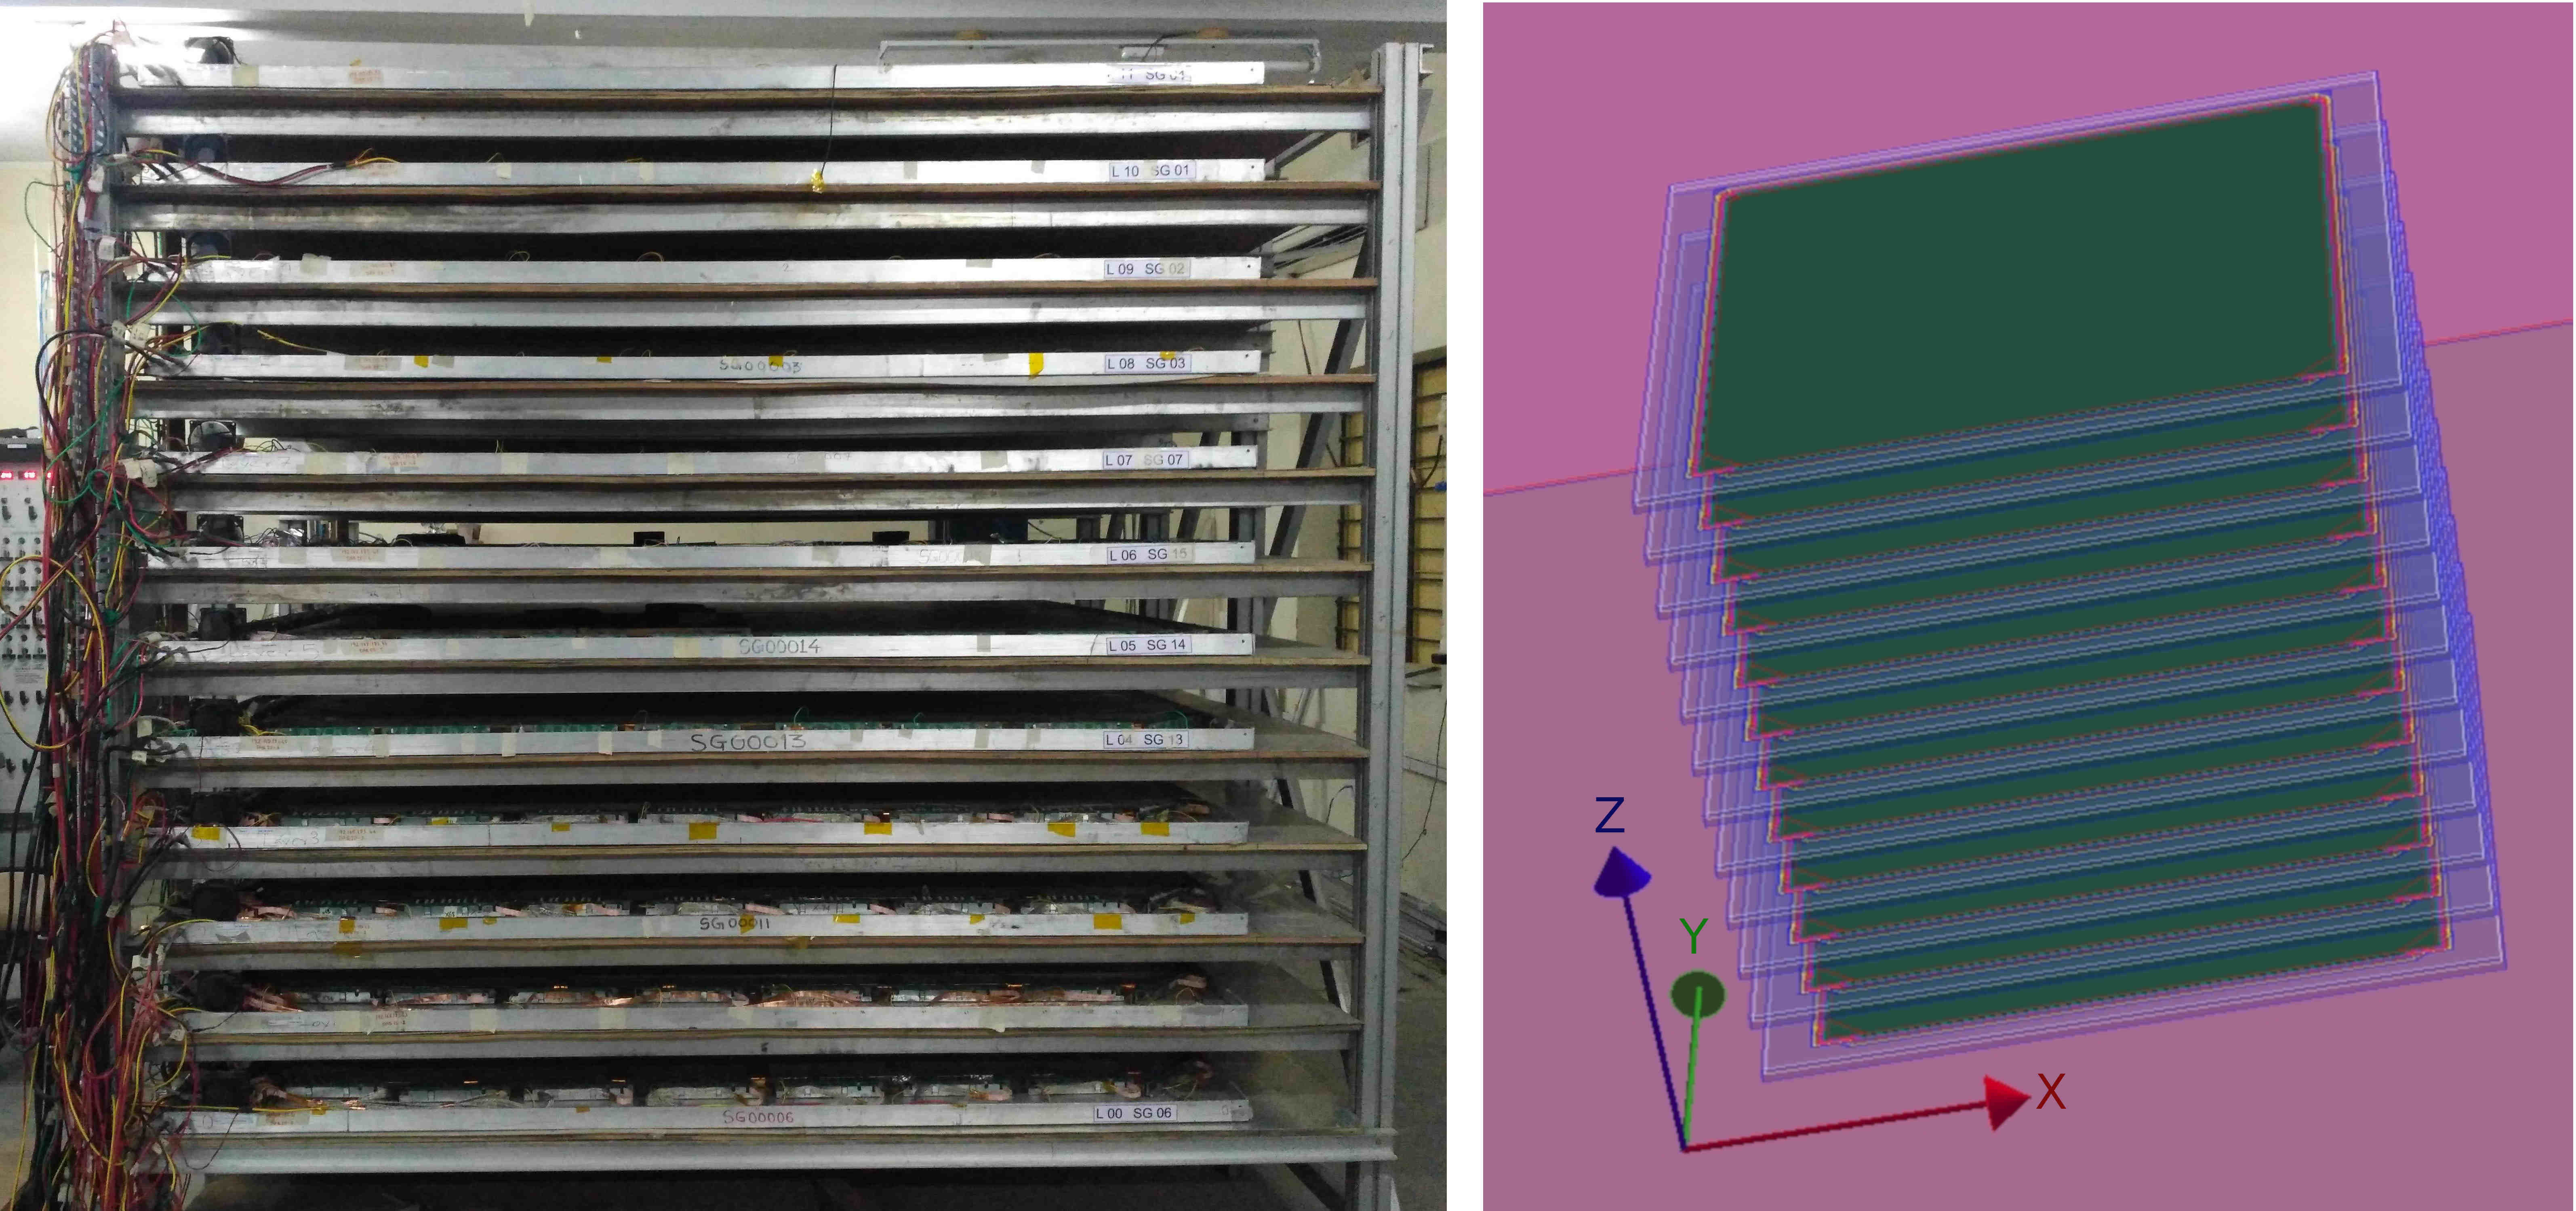
\includegraphics[width=0.99\linewidth]{ABlockStackiDAQ_new.jpg} 
  \caption{The detector stack with 12 layers of RPCs where the
    $X$-axis of the detector is making an angle of $-10^\circ$ with
    the geographic south, (left) experimental setup and (right) Geant4
    detector geometry of stack.}
  \label{fig:stack}
\end{figure}
An RPC gap is made of two glass electrodes of thickness 3\,mm with
a gap of 2\,mm between them. Uniform gap between these two electrodes
is maintained using an array of 2\,mm thick poly-carbonate buttons.
The glass gap is sealed on the outer edges to make it air-tight.
A non-flammable mixture of gas is continuously
flown inside the glass gaps via strategically placed nozzles.
This mixture of gasses serves as the active medium of the detector.
The RPCs are operated in avalanche mode. In this case, the mixture of
gases consists of R134a (95.2\%), iso-C$_4$H$_{10}$ (4.2\%) and
SF$_6$ (0.3\%). Both the outer surfaces of the glass gap are coated
with a thin layer of graphite. The RPCs are operated by applying
a differential supply of $\sim\:\pm$\,5\,kV to the graphite layers to
achieve the desired electric field. A small variation in applied HV is
  due to the variation of gain in different RPC. The target gas inside the RPCs gets
ionised by the transit of charged particles. This ionisation eventually
evolves into an avalanche in the presence of the high electric field
between the glass electrodes. The avalanche in the RPCs induces
signals in the two orthogonal pickup panels placed on both sides of
the glass gaps labelled as X-side (bottom) and Y-side (top). The pickup
panels are made of parallel copper strips of width 28\,mm with 2\,mm
gap between two consecutive strips. The RPCs used in this detector
stack are of the size of 1790\,mm\,$\times$\,1890\,mm. There are
60 strips on the X side and 63 strips on the Y side for each layer.

The induced signals from the pickup strips are amplified and
discriminated by a charge sensitive NINO\cite{nino}
amplifier-discriminator board. Only in layer 11 (topmost layer),
ANUSPARSH ASIC\cite{anusp} which is a CMOS, 8-channel,
high speed, low power amplifier-discriminator designed for
avalanche mode of operation for RPCs is used to study its performance.
The discriminated signals from these boards are passed
to the FPGA-based RPCDAQ-board.
The individual signals from every 8$^{th}$ strips are \emph{OR}ed
to get pre-trigger signals (S0 to S7), which are passed to the Trigger
system module via Signal Router Board. The four-fold coincidence is done
for X- and Y- sides independently in the Trigger Logic Boards.
The Global Trigger is then generated by the Global Trigger Logic Board
(GTLB) by \textit{OR}ing the coincidences formed in X- and Y-side.
The trigger scheme of the detector setup contributed by 4 RPC layers is
illustrated in the Figure~\ref{fig:trigger}.
\begin{figure}[h]
  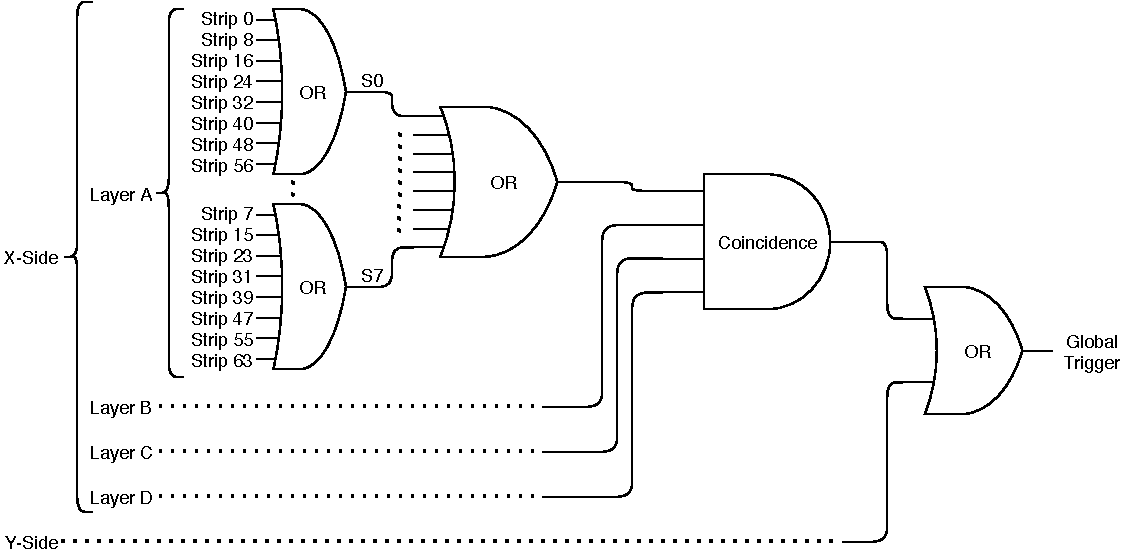
\includegraphics[width=1.0\linewidth]{DAQTriggerScheme.pdf} 
  \caption{Trigger Scheme of the Detector Setup.}
  \label{fig:trigger}
\end{figure}
%% The individual signals from every 
%% 8$^{th}$ strips are \emph{OR}ed to get pre-trigger signals (S0 to S7).
%% The 1-fold (S0+S1+...S7), 2-fold (S0.S1+S1.S2+..S6.S7),
%% 3-fold (S0.S1.S2+....S5.S6.S7) and 4-fold
%% (S0.S1.S2.S3+....S4.S5.S6.S7) signals created by RPCDAQ are passed
%% to the Trigger system module via Signal Router Board. The Global
%% Trigger is generated by Global Trigger Logic Board based (GTLB)
%% on X- or Y-plane with at least one strip hit within
%% 100\,ns coincidence window. The coincidence is done for X and Y plane
%% independently and the final trigger can be generated by GTLB by OR
%% of Trigger in X- or Y-plane. The higher order trigger configurations
%% are useful where neutral-current interaction are expected within the
%% detector generating tracks with shorter tracks but higher multiplicity.
%% However only 1-fold signal is used to generate the trigger in the
%% current study as we are expecting only muon-events in the detector
%% which creates longer tracks. 

The hit signals in the RPCDAQ board
stretched to 1\,$\mu$s to overcome trigger latency of 770\,ns from
Trigger System to RPCDAQ. Based on the arrival of trigger signals to
RPCDAQ, the event signals are latched and sent to the Data Concentrator
and Event Builder via Network Switch. The trigger system's `dead-time'
is set at 500\,ns after generation of a trigger to process and store %GMA is it 500ns ?
the triggered event.
The flow of signals in the detector setup is shown in the
Figure~\ref{fig:sigflow}.
\begin{figure}[h]
  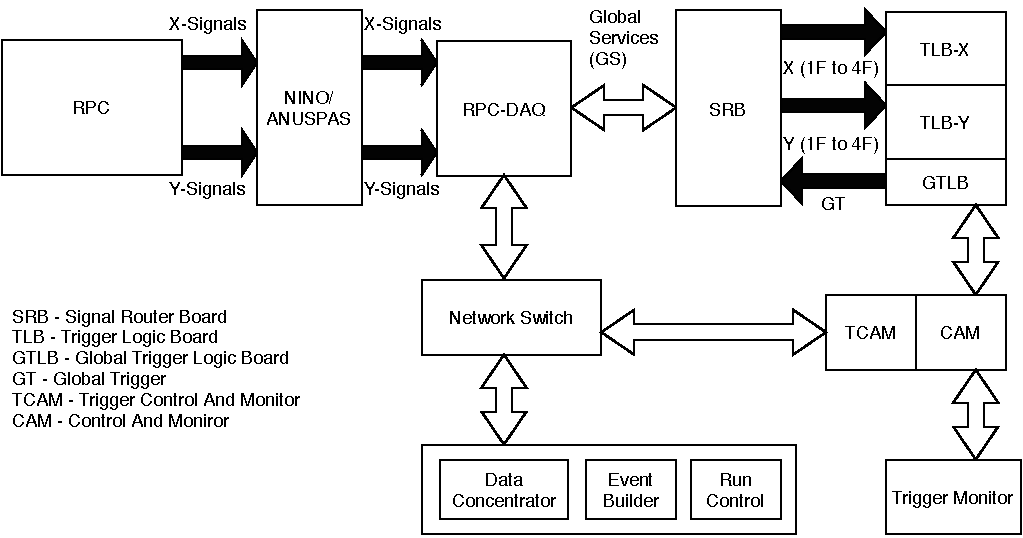
\includegraphics[width=1.0\linewidth]{DAQSchemeNewElectronics.pdf} 
  \caption{The Flow of Signals in the Detector Setup.}
  \label{fig:sigflow}
\end{figure}
The detailed description of signal processing and the Data Acquisition
system (DAQ) can be found in \cite{elec1}. The present work is based
on the coincidence of pre-Triggered signals from layers 4, 5, 6 and 7
within a coincidence window of 100\,ns. While the layers in the middle
portion of the detector are used to form the trigger, the layers in
both the top and bottom portions of the detector also contributes in
forming an event, which in turn maximises the length of the track in
the detector.
%% The 1-Fold signals
%% from layers 4, 5, 6 and 7 are used as trigger to record the cosmic
%% events used in the present work.

The stretched signals get latched for recording when the trigger
reaches the RPCDAQs. Ideally, the signals occurring only within the
coincidence window should get latched. But for this setup, the signals
for any other particles as well as noise occurred outside the
coincidence window also may get recorded due to stretching of the hit
signals and trigger latency. A generalised timing diagram of an event
which includes the hits from two particles is shown in the
Figure~\ref{fig:timingdiagram} to illustrate this.
\begin{figure}[h]
  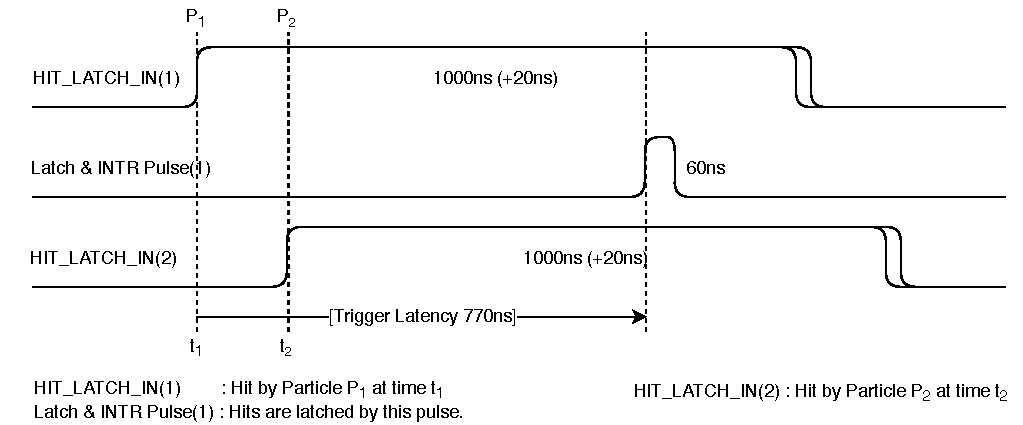
\includegraphics[width=1.0\linewidth]{TimingDiagram-TimeSimple.pdf} 
  \caption{Timing diagram of an event.}
  \label{fig:timingdiagram}
\end{figure}
If a particle, generating the trigger, has passed through the
detector at time $t_{1}$, then all other signals within the period of
$t_{1}$ to $t_{1}+770$\,ns also get recorded due to the trigger latency
of 770\,ns. The signals generated within the time period
$t_{1}-230$\,ns to $t_{1}$\ also get recorded as well but only in
the following situations.
\vspace*{-10pt}
\begin{itemize} \itemsep -5pt
\item \textbf{Case~1:} The hits generated by the other particle did
  not satisfy the trigger criteria.
\item \textbf{Case~2:} The hits generated by the other particle
  satisfied the trigger criteria, but failed to generate a trigger
  as it occurred within the `dead-time' of the trigger system.
\item \textbf{Case~3:} The hits generated by any of the particles in
  the event did not satisfy the trigger criteria individually.
  But hits generated by both particles altogether satisfy the trigger
  criteria.
\end{itemize}

An event typically contains hit information (one logic bit per strip
indicating the signal in that strip) for each strip and 16 time
signals for each layer; 8 for X-side and other 8 for Y-side.
One TDC (Time-to-Digital~Converter) channel with least-count of 0.1\,ns
records time signals coming from every alternating 8$^{th}$ strips
(S0 to S7). Approximately 250 millions of cosmic ray events
recorded in the detector during the total observation period between
August 23, 2017 to September 8, 2017 with a trigger rate of
$\sim$230\,Hz are used for the analysis.


\section{Monte-Carlo Simulation} \label{sec:montecarlo}
The Monte-Carlo Simulation for this study has been executed in
two stages. The Extensive Air Shower (EAS) has been simulated
by the CORSIKA simulation package\cite{corsika763}. The information
of daughter particles generated by the EAS at the earth's surface
level has been extracted and used as the input data to the detector
simulation. The detector simulation has been executed with the help
of the GEANT4 toolkit\cite{geant4}.

\subsection{Extensive Air Shower}
The CORSIKA (COsmic Ray SImulations for KAscade) is developed to study
the evolution of the EAS in the atmosphere created by primary cosmic
ray. Though the CORSIKA has been developed initially for a specific
experiment, this package is now developed into a tool that is used
by many groups studying cosmic rays and EAS.
In the current study, existing extrapolations of hadronic interaction
models of high energy particles in the EAS are based on
various theoretical models, which have large uncertainties.
The current experimental data at the collider experiments is
insufficient to verify the extrapolation of the hadronic interactions
at very high energies. In the CORSIKA package, several different
hadronic interaction models are available. In this study, for
simulating the behaviour of hadrons for higher energy range,
the QGSJET (Quark Gluon String model with JETs)\cite{corsika763} has
been adopted and for the low energy range (less than 80\,GeV in
laboratory frame), the GHEISHA model has been used.

In this study, the primary cosmic ray shower has been simulated using
the CORSIKA(v7.6300) Package. The energy of the primary rays in the
CORSIKA is generated using the power-law spectrum, $E^{-2.7}$, within
the energy range of \mbox{$10$--$10^{6}$\,GeV} for different primaries
(H, He, C, O, Si and Fe). The zenith and azimuth angle of the primary
cosmic particles are generated uniformly within the range of
\mbox{$0$--$85^\circ$} and \mbox{$0$--$360^\circ$}, respectively. The
rigidity cutoff due to the earth's magnetic field has been implemented
as per the location of the detector. The minimum energy cutoffs for
secondary hadrons, muons, electrons and photons in the simulation are
kept at 50\,MeV, 10\,MeV, 1\,MeV and 1\,MeV, respectively. These cutoff
values are much smaller than the minimum momentum cutoff for
the charged particles in the vertical direction,
\mbox{$\sim 110$\,MeV}, which is mainly due to 22\,cm of concrete
roof of the building where the detector is placed. The momentum
spectra of secondary charged particles generated by the CORSIKA
simulation is shown in the Figure~\ref{fig:momin}.
%GMA four plots for all those particles with lower range 1 MeV
%% \begin{figure}[h]
%%   \centering
%%   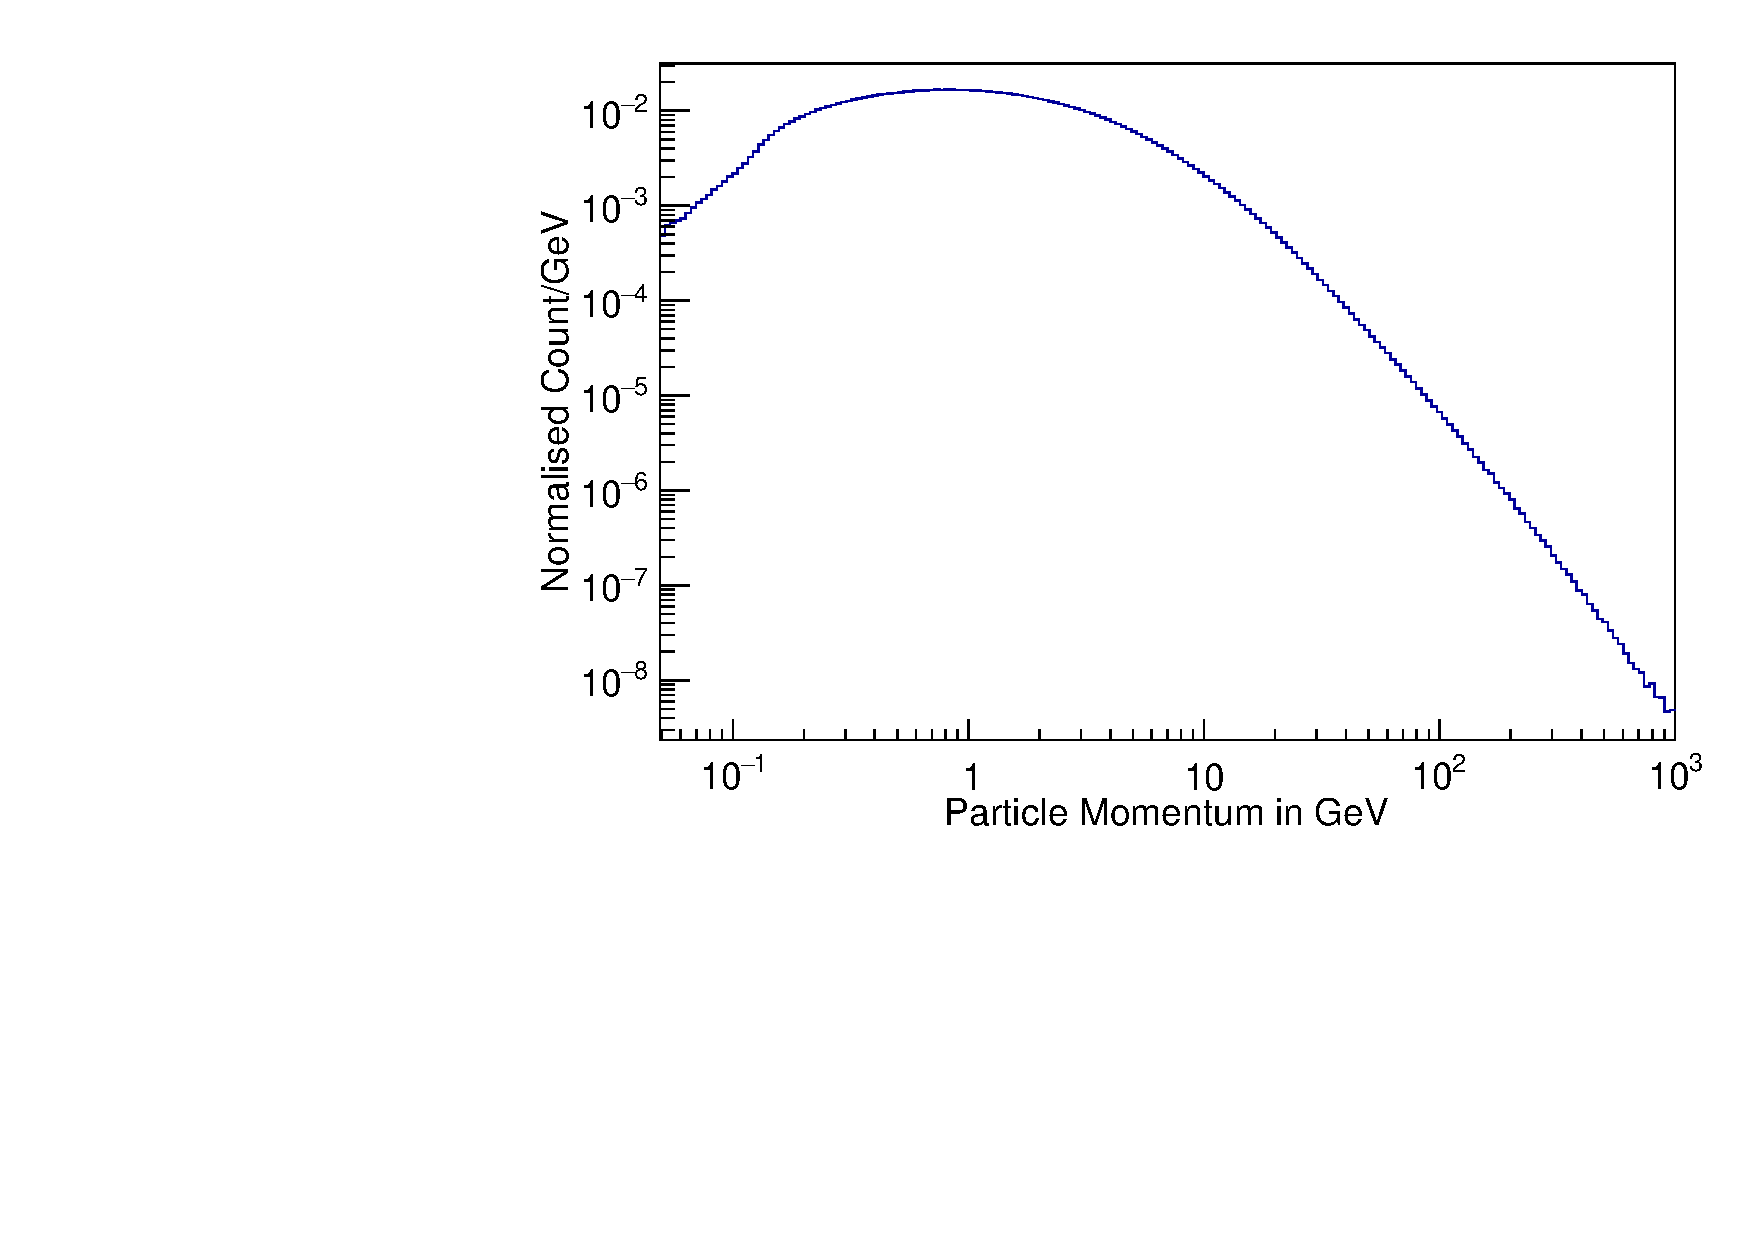
\includegraphics[width=0.6\linewidth]{momin_reco_1.pdf} 
%%   \caption{CORSIKA generated momentum of charged particles at observation level.}
%%   \label{fig:momin}
%% \end{figure}
\begin{figure}[h]
  \centering
  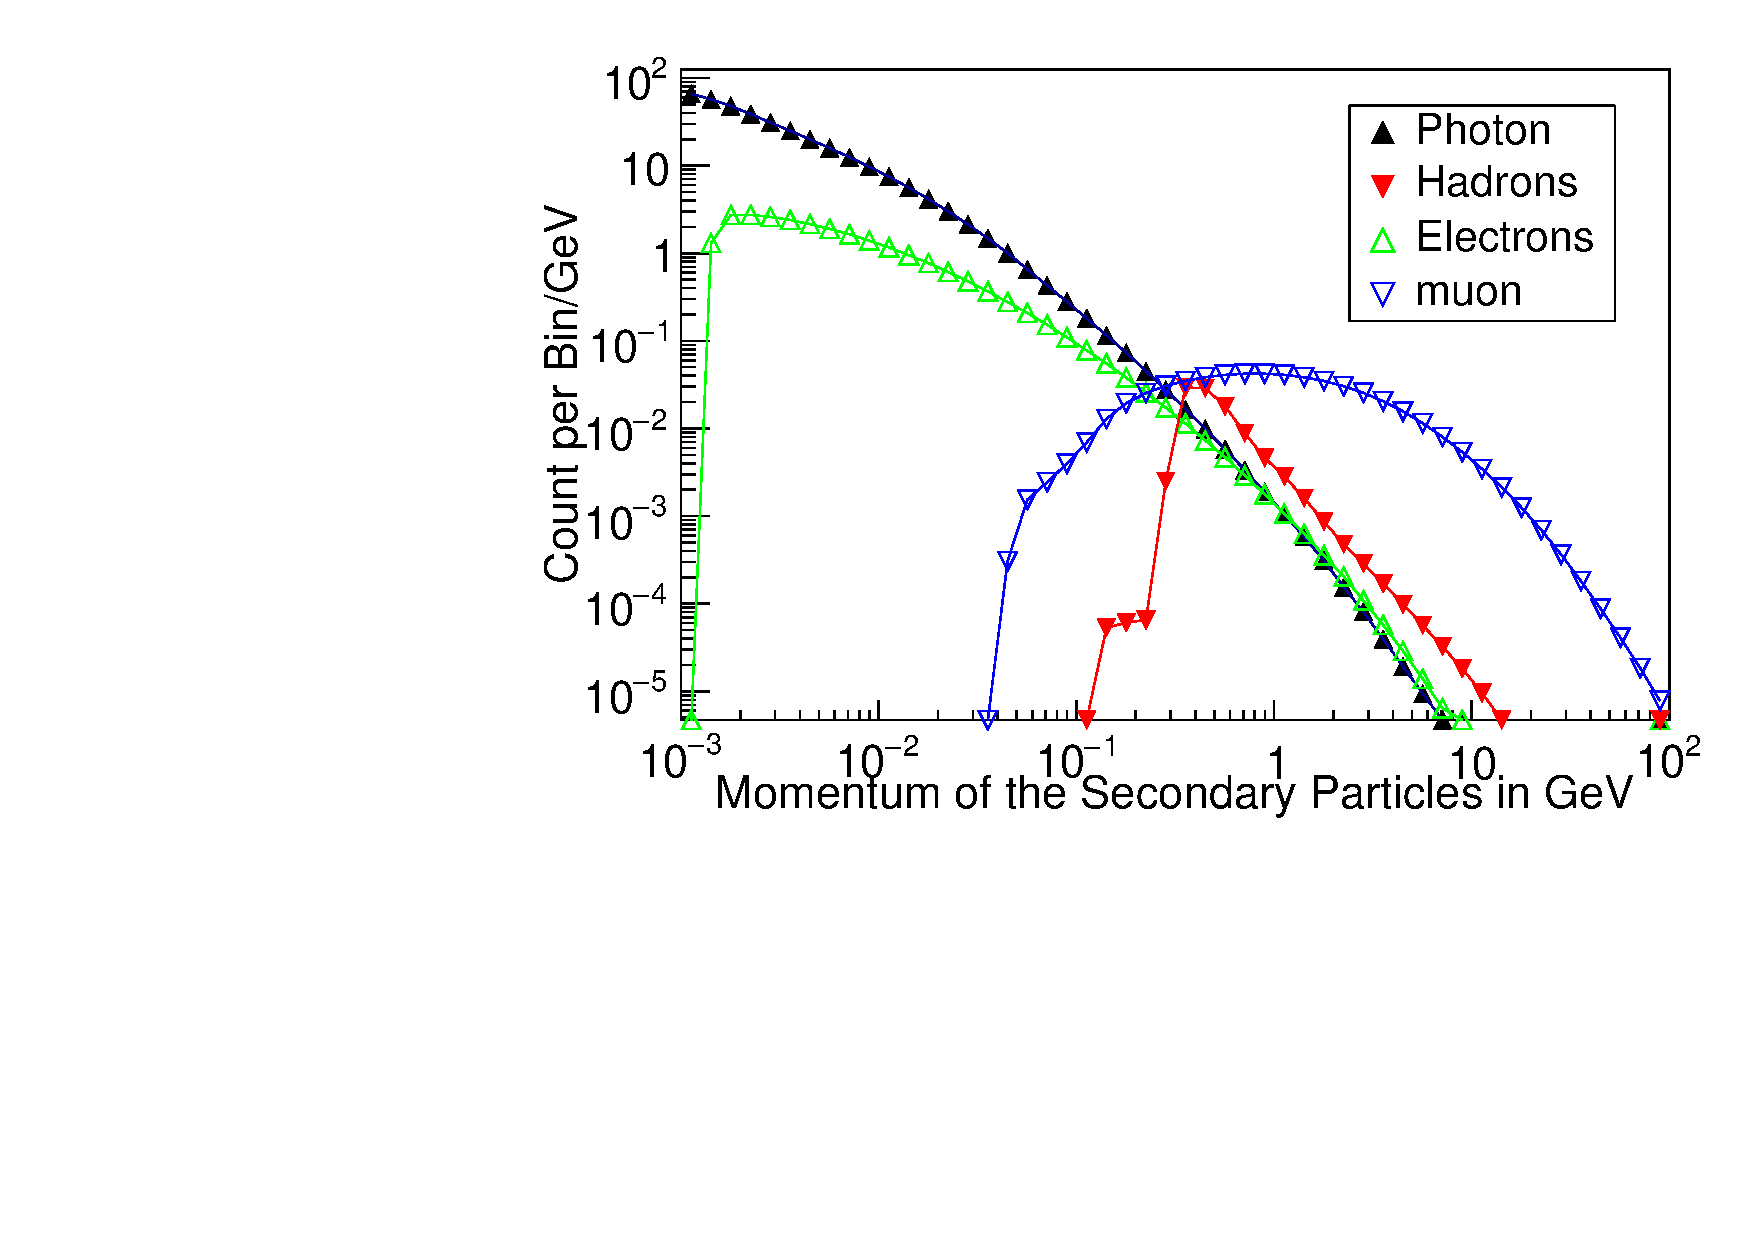
\includegraphics[width=0.6\linewidth]{corsika_secondary_energy.pdf} 
  \caption{CORSIKA generated momentum of secondary particles at
    observation level.}
  \label{fig:momin}
\end{figure}

The secondary particles generated by the CORSIKA which are reaching
the observation surface are provided as an input to the detector
simulation. The observation plane has been divided
into squares of the size of 2\,m\,$\times$\,2\,m which is shown in the
Figure~\ref{fig:eas}.
\begin{figure}[h]
  \centering
  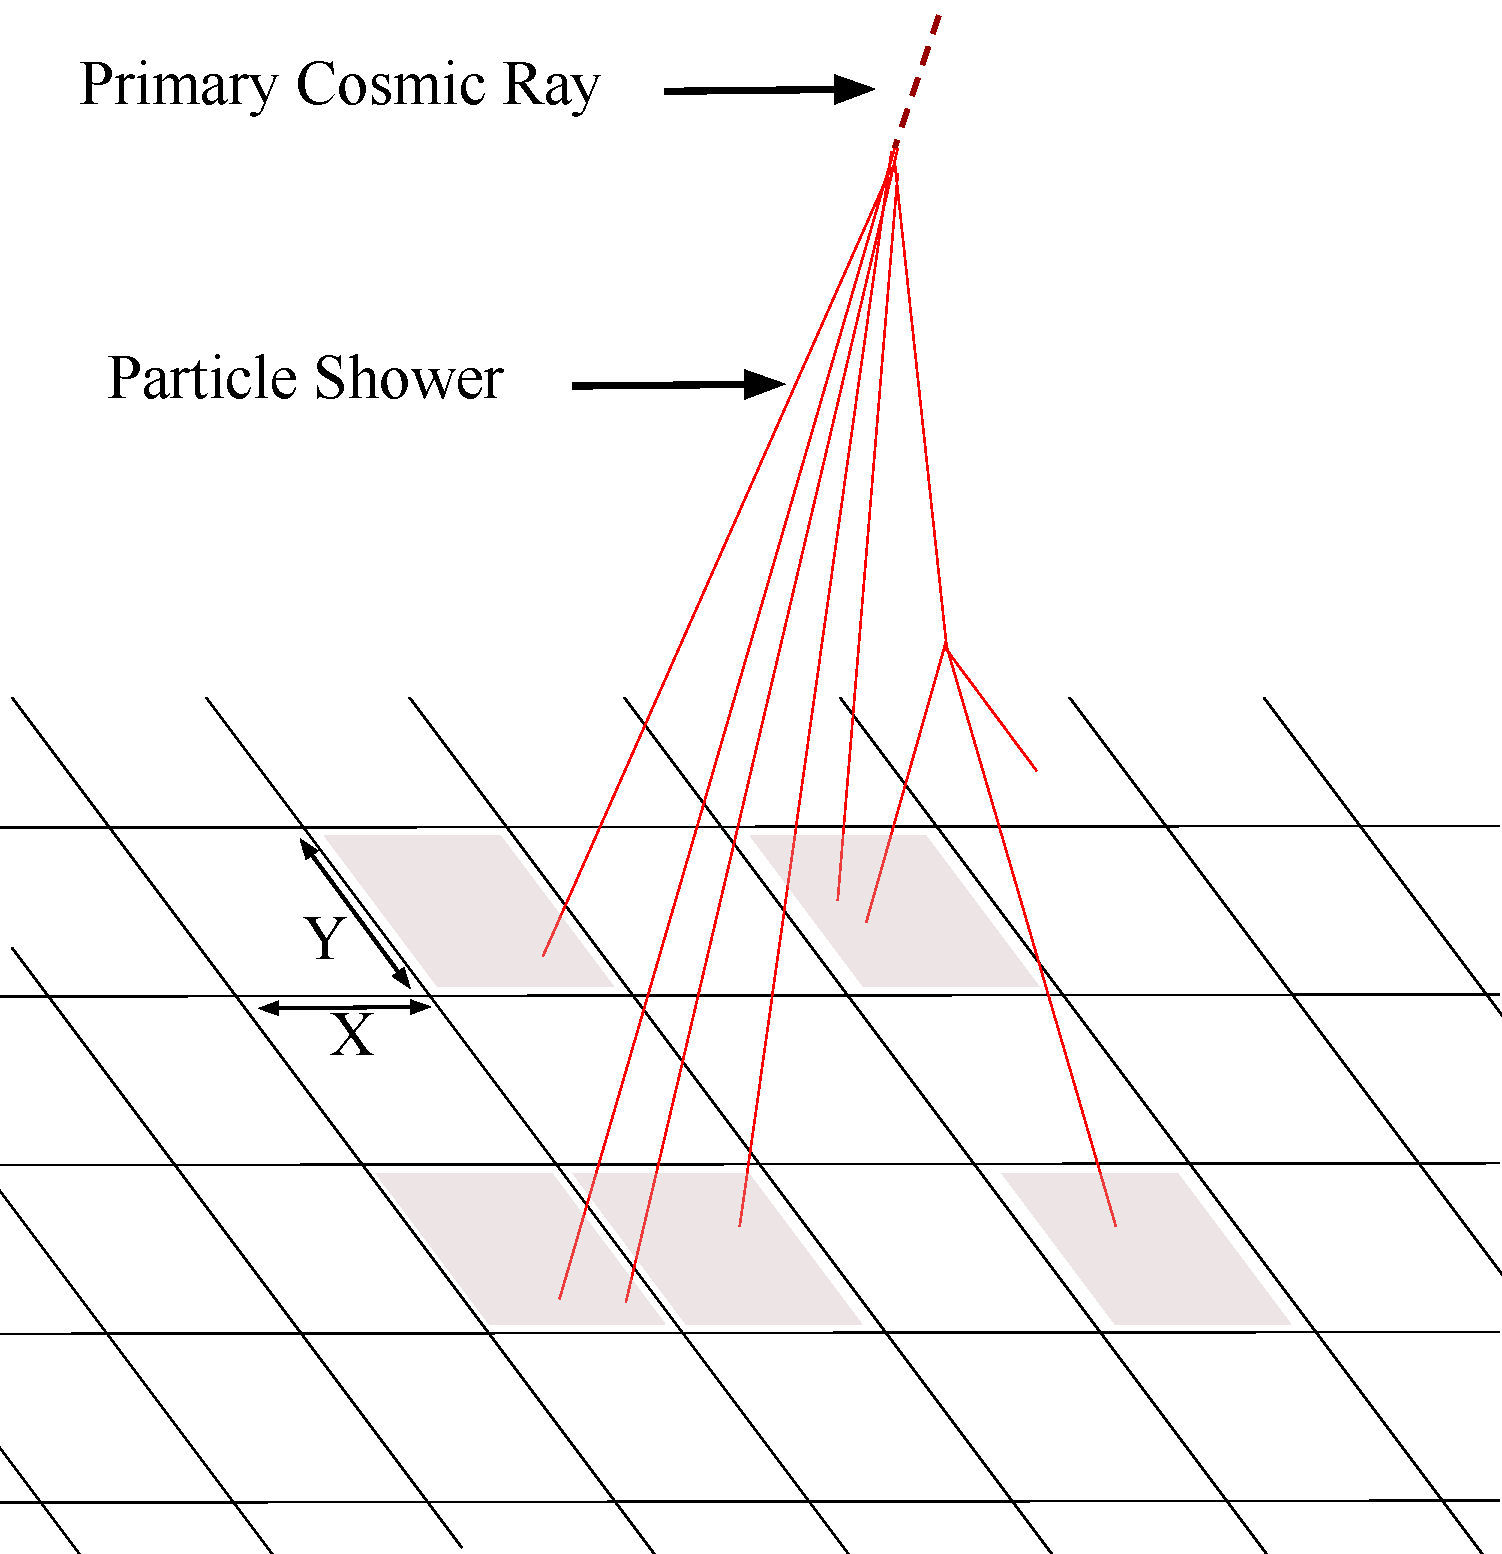
\includegraphics[width=0.6\linewidth]{EAS.pdf} 
  \caption{Shower of particles initiated by primary cosmic ray
    reaching observation surface.}
  \label{fig:eas}
\end{figure}
An event is formed using the information of the particle(s) reaching
to each of these squares shown as shaded region in the
Figure~\ref{fig:eas}.


\subsection{Detector Simulation}
The detector simulation has been accomplished using the
GEANT4(v4-10.0.2) toolkit. The events generated in the CORSIKA
simulation are propagated event-by-event in the detector simulation.
A realistic depiction of the detector setup including the building
where the detector is housed has been constructed in the GEANT4
environment. The materials of the various detector components and
the laboratory buildings are chosen based on the knowledge of the
setup. The uncertainty of the material budget is taken as a systematic
error. The physics processes of matter-particle interactions 
%GMA explicitly mention which models are used for Hadronic and EM interactions
like electromagnetic, ionisation, decay and hadronic interactions,
which are available within the GEANT4 toolkit are considered in the
simulation.

The various detector parameters (efficiency, noise, strip
multiplicity and resolution) are calculated using the cosmic rays
passing through the detector stack.
The current setup is a tracker type detector consisting of 12 layers
of RPCs. When one layer of the setup is studied for the detector
parameters, the rest of the layers in the setup serve as the tracker
for the passing particles. Since the layers forming the coincidence
cannot be studied for the detector parameters, the data sets with two
more different trigger combinations (using layers 1,2,3,4 and 7,8,9,10
to form coincidences) of the duration of one day, are used in order
to study all the RPCs in the setup.

The efficiency of a RPC gap is defined as the probability of getting
a signal from a RPC when a particle has passed through it.
Each of the RPC detectors can be divided into a matrix of pixels of
size 3\,cm$\times$\,3\,cm. The efficiencies of each of the pixels
are calculated and represented as the efficiency map for each of the
RPCs. The track(s) of the particle(s) in an event is fitted with the
straight line by excluding the RPC layer being studied from the fit.
For each pixel in that RPC layer, the total number of particles passed
through it is estimated from the extrapolated position in that layer.
The ratio of the number of events with valid hit signal in X- (or Y-)
strips of that pixel to the total number of particles passed through
it is taken as the efficiency for the X- (or Y-) side of that pixel.
The noise in a RPC is defined as the hits occurred farther from the
expected position of the passing particle. The strip multiplicity
profile is defined as the probability of sharing signal between
neighbouring strips with respect to the hit position from the centre
of the strip. The strip multiplicity is discussed in the next section.
A detailed study of these parameters are presented in \cite{pethu1}.
The efficiency map, noise and strip multiplicity
profile for one of the RPCs in the stack is shown in the
Figure~\ref{fig:layer2y}.
\begin{figure}[h]
  \centering
  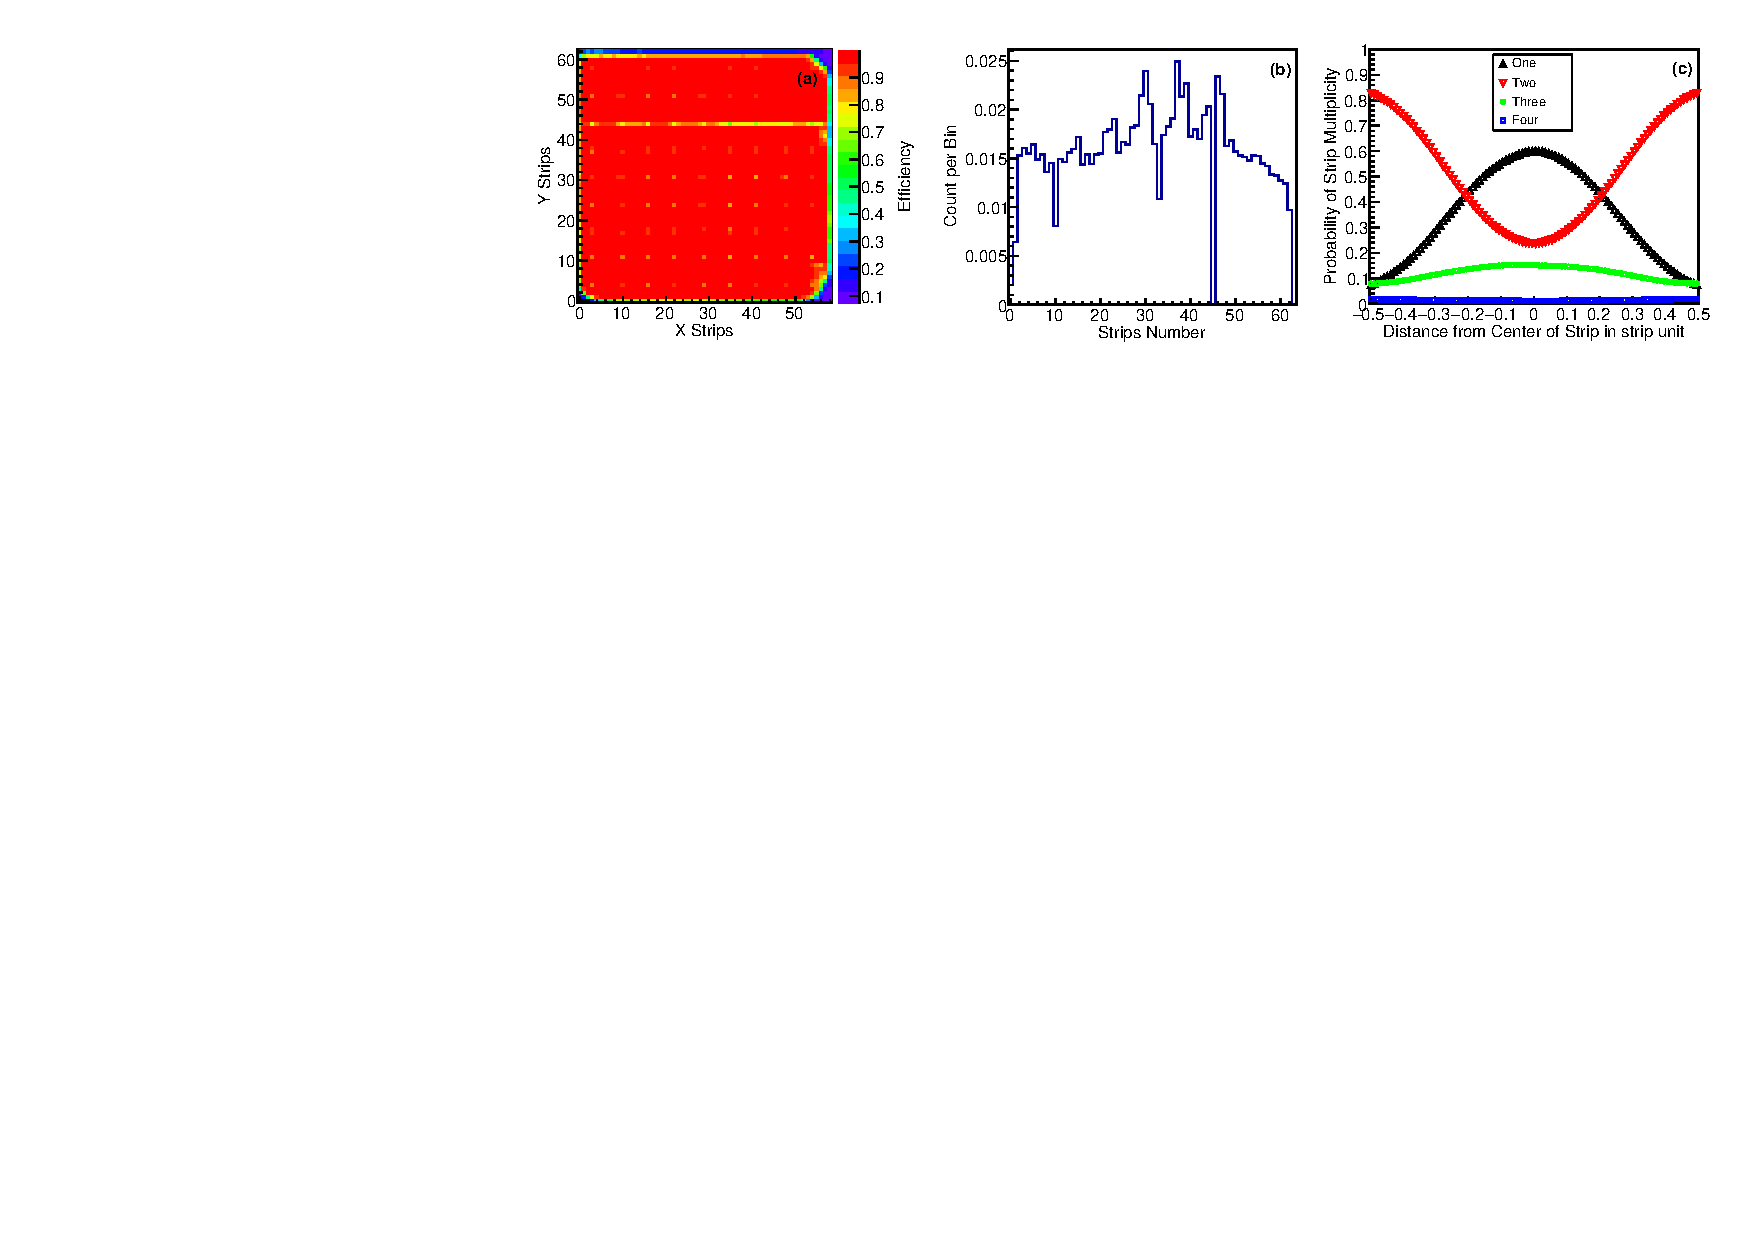
\includegraphics[width=1.\linewidth]{layer2properties.pdf} 
  \caption{(a) Efficiency, (b) Noise and (c) Multiplicity profile of
    Y side of Layer-2 RPC gap.}
  \label{fig:layer2y}
\end{figure}
These observed detector parameters are included in the digitisation
stage of the detector simulation. Both the events from the observed
cosmic ray data and the detector simulation are reconstructed using
an algorithm based on Hough Transformation which is discussed in the
next section.

\section{Event Reconstruction and Data Selection}\label{sec:reconstrction}
For the event reconstruction, the strip hits are
analysed separately, in the 2-dimensional projections namely,
\mbox{X--Z} and \mbox{Y--Z} sides. During the passage of a charged
particle through a RPC gap, the number of strips on which signal is
induced depends on the gain of the gas gap. This sharing of the induced
signal between the neighbouring strips is the main reason for the
observed strip multiplicity shown in the Figure~\ref{fig:layer2y}(c).
In order to prepare the events for this study, the consecutive strips
which have recorded signals are clubbed together to form a cluster.
During the study, the position resolution is calculated for different
strip multiplicities of 1, 2, 3, and 4 and the values observed are
$\sim$6\,mm, $\sim$8\,mm, $\sim$12\,mm and $\sim$22\,mm respectively.
The position resolution for strip multiplicities more than four is
larger than the pitch of the strip (3\,cm). So in this study,
the clusters of hits with more than 4 multiplicities are neglected
as the position resolution for higher multiplicities is found to be
the worst.
A layer which has more than 15 strip hits and/or more than 10 clusters
is tagged as `noisy layer' and not considered in the track
reconstruction. The first criterion has been chosen near the maximum
number of possible hits if 4 tracks pass through a RPC.
In fact, the maximum number of tracks reconstructed in an event is 4
which is discussed in the Result section. The second criterion is set
at the first criterion divided by the average strip multiplicity
$\left(\sim 1.5\right)$ in the detector stack to reject noisy events
passed through the first criterion.
An event which has more than 3 noisy layers is considered as `noisy
event' and discarded. This criterion is set at 3 layers which is 25\%
of maximum layers available for the event reconstruction. This
criterion has been set by considering the performance of the
reconstruction method and number of events lost due to this criterion.

In the first step of track reconstruction, the clusters associated
with different tracks are found and grouped using the method of Hough
Transformation\cite{hought1,hought}. The equation of the straight line,
used to find the association between the hits, is given as,
\begin{equation}
  r=z\cos\theta+x\left(/y\right)\sin\theta. \label{eq:hough}
\end{equation}
The \mbox{$r$-$\theta$} plane (also called as Hough Space) is
populated using the concept of Cellular Automaton\cite{cellular}.
For a sample event shown in the Figure~\ref{fig:houghPl}(a),
the populated \mbox{$r$-$\theta$} plane is presented in the
Figure~\ref{fig:houghPl}(b).
\begin{figure}[h]
  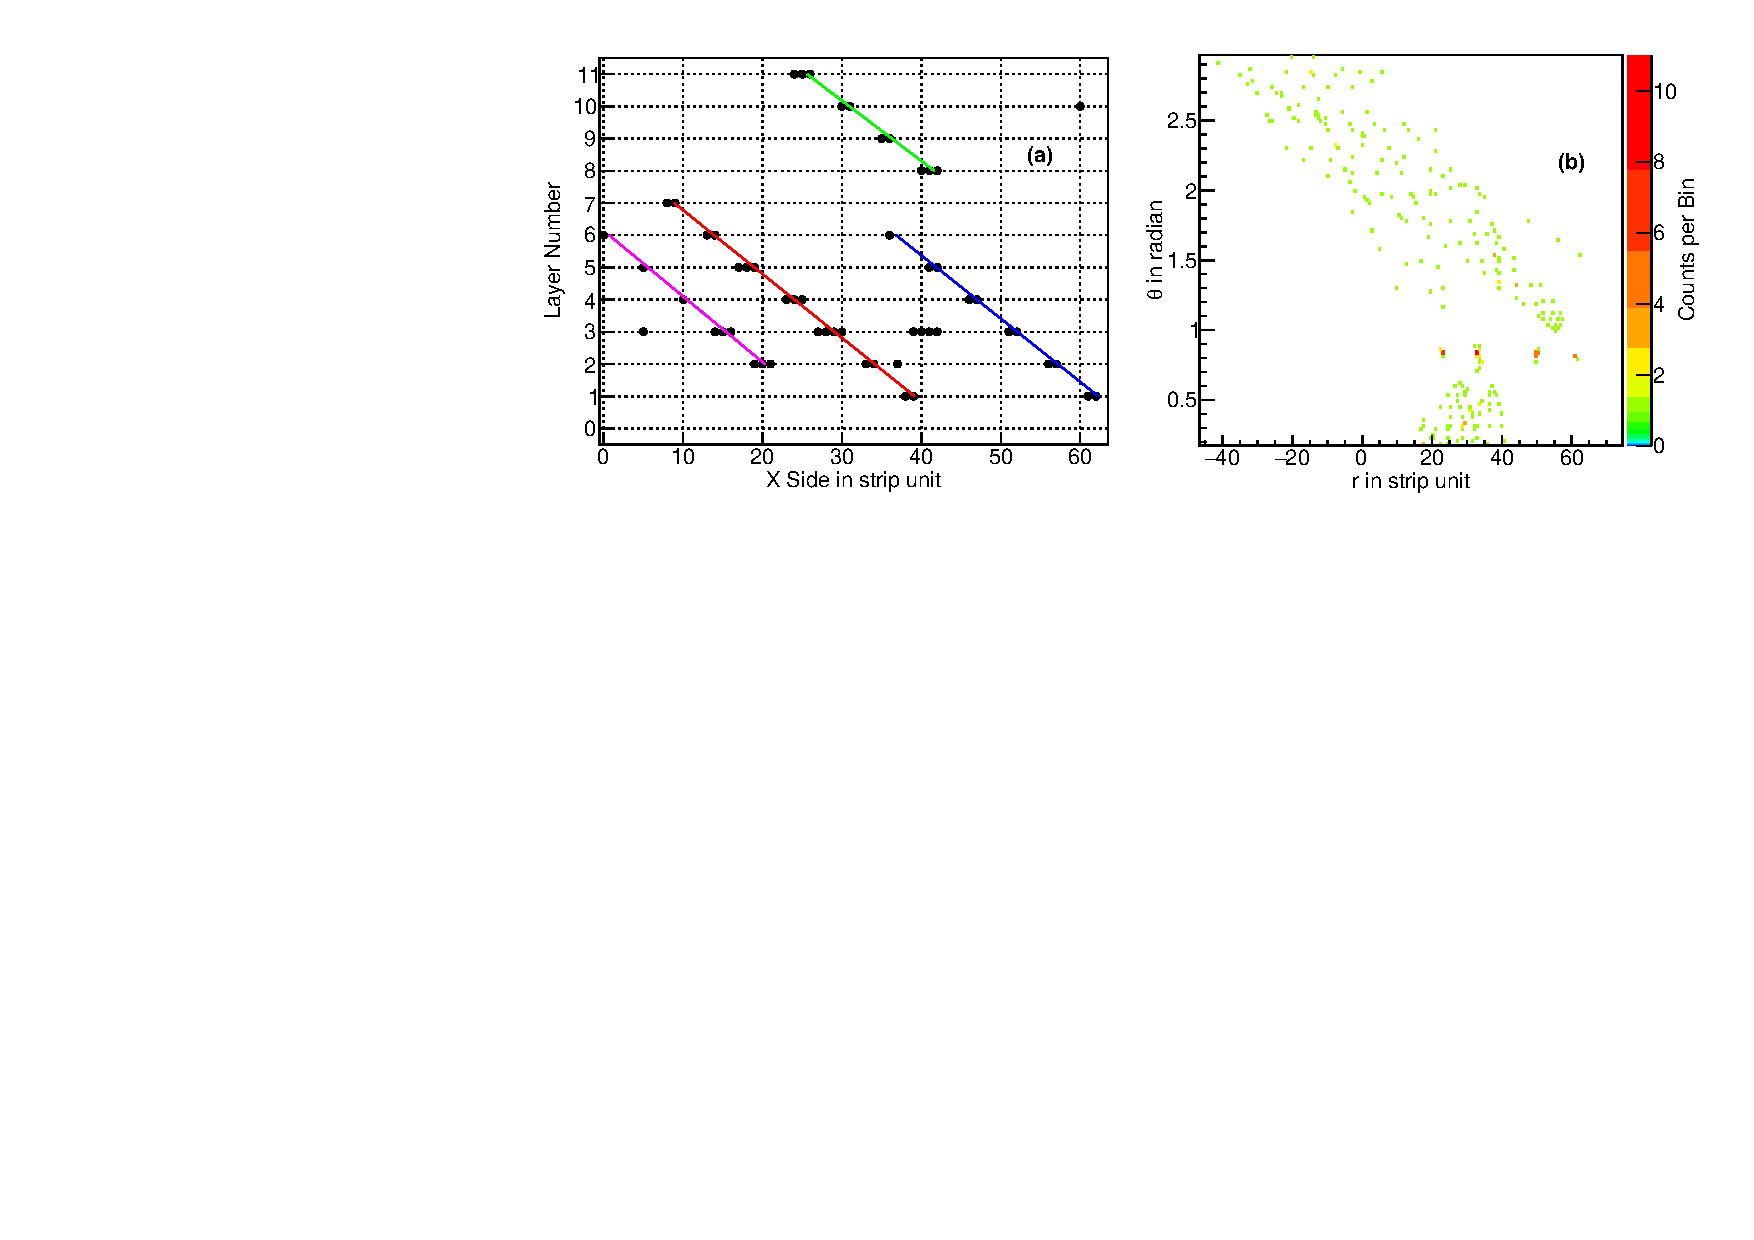
\includegraphics[width=1.0\linewidth]{hough_Plane.pdf} 
  \caption{(a) Projection of an event in the detector and
    (b) populated $r$-$\theta$~plane using this event.}
  \label{fig:houghPl}
\end{figure}
The advantage of using Cellular Automaton technique is the significant
reduction of computation time to find a trajectory in the event.
This method can detect all the tracks avoiding the noise hits as
shown in Figure~\ref{fig:houghPl}(a).

The tracks identified using the Hough Transformation are then
fitted by a straight line given by the equation,
\begin{equation}
  x\left(/y\right)=mz+c \label{eq:plain}
\end{equation}
where $m$ and $c$ are the slope and the intersect, respectively.
The number of detector layers in the fit and $\chi^{2}$/ndf of
the fit are shown in the Figure~\ref{fig:chi2ndf}(a) and
\ref{fig:chi2ndf}(b) respectively.
\begin{figure}[h]
  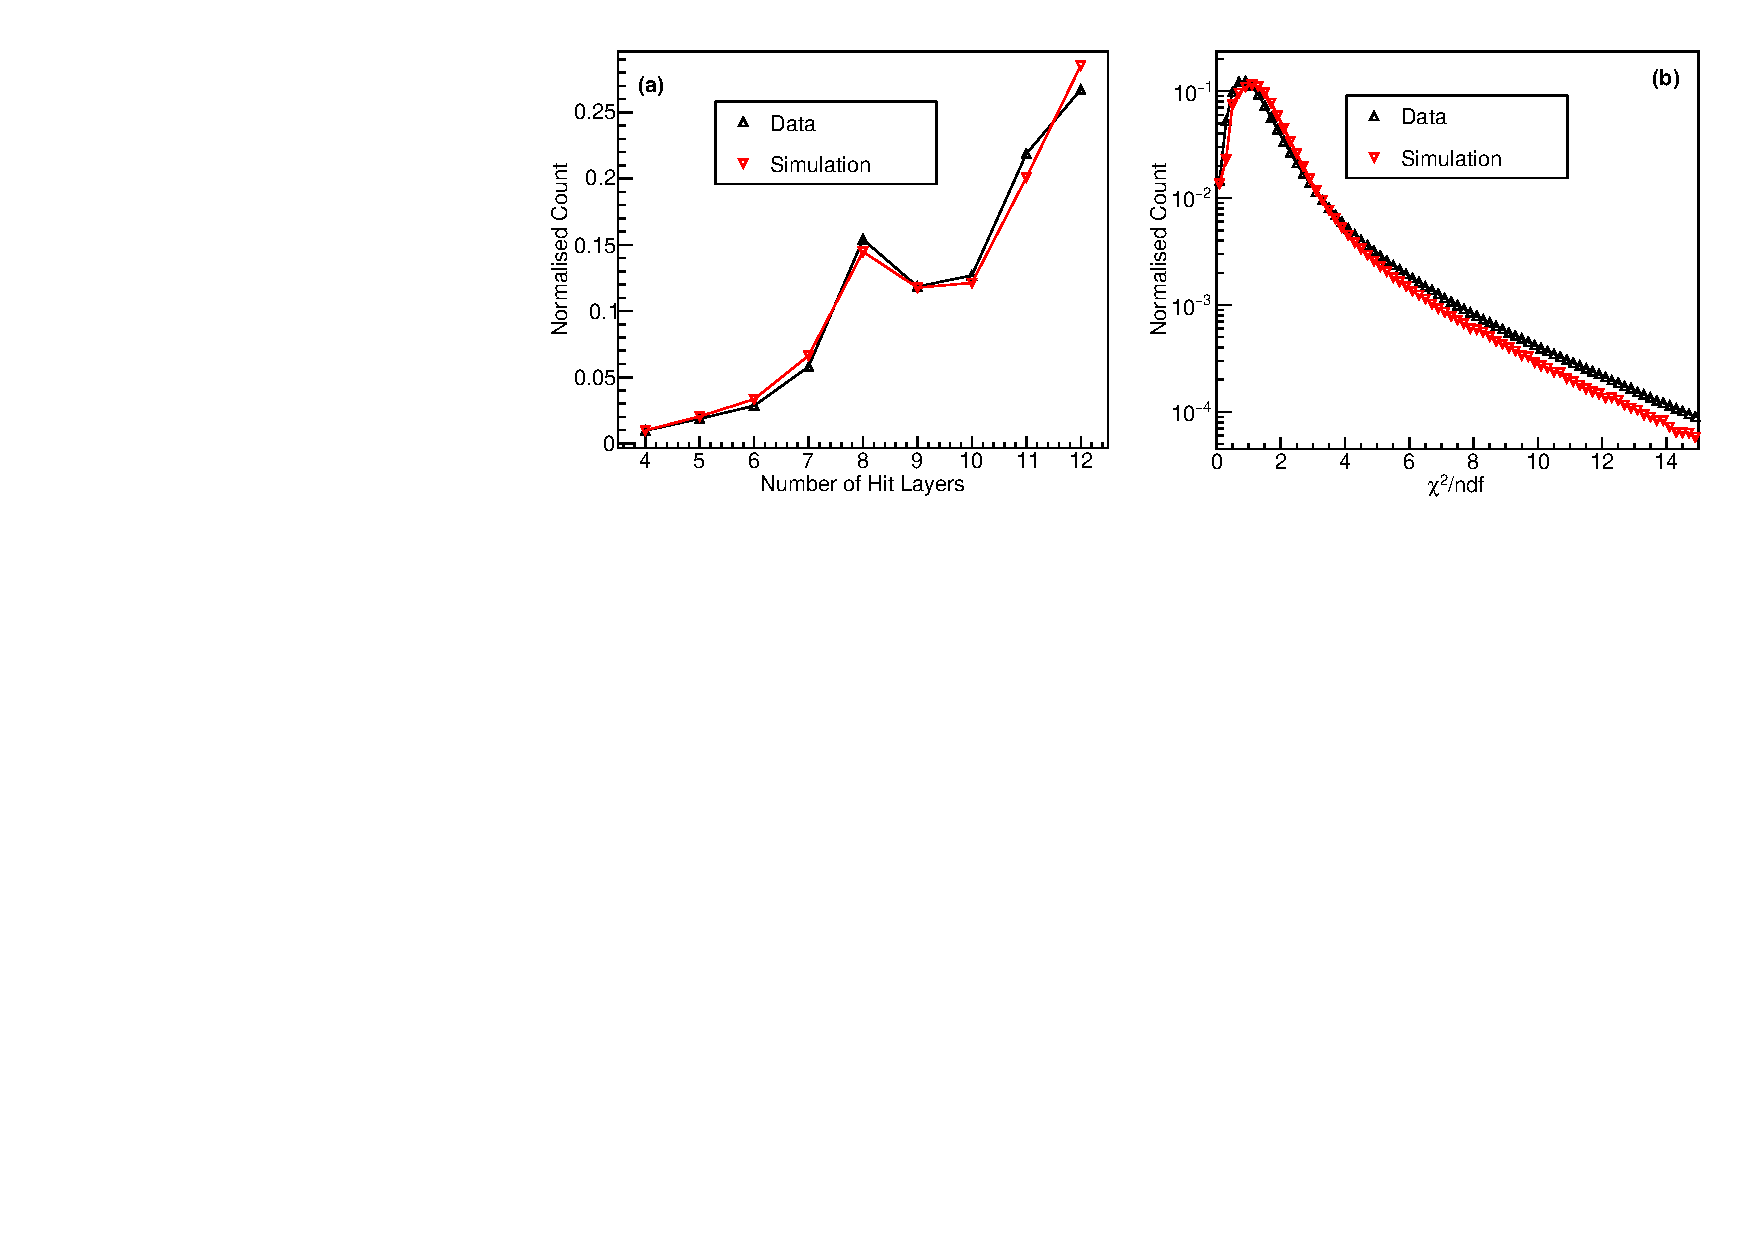
\includegraphics[width=1.0\linewidth]{chi2ndf_compare_all.pdf} 
  \caption{(a) Number of hit layer and
    (b) $\chi^2$/ndf of straight line fit.}
  \label{fig:chi2ndf}
\end{figure}
A track is considered as properly reconstructed if the $\chi^{2}$/ndf
is less than 10 and there are more than 4 layers in the track.
The reconstruction efficiency is defined as the ratio of the number
of events with at-least one reconstructed track to the total number
of triggered events. The reconstruction efficiency as a function of 
time is shown in the Figure~\ref{fig:stackineffi}.
\begin{figure}[h]
  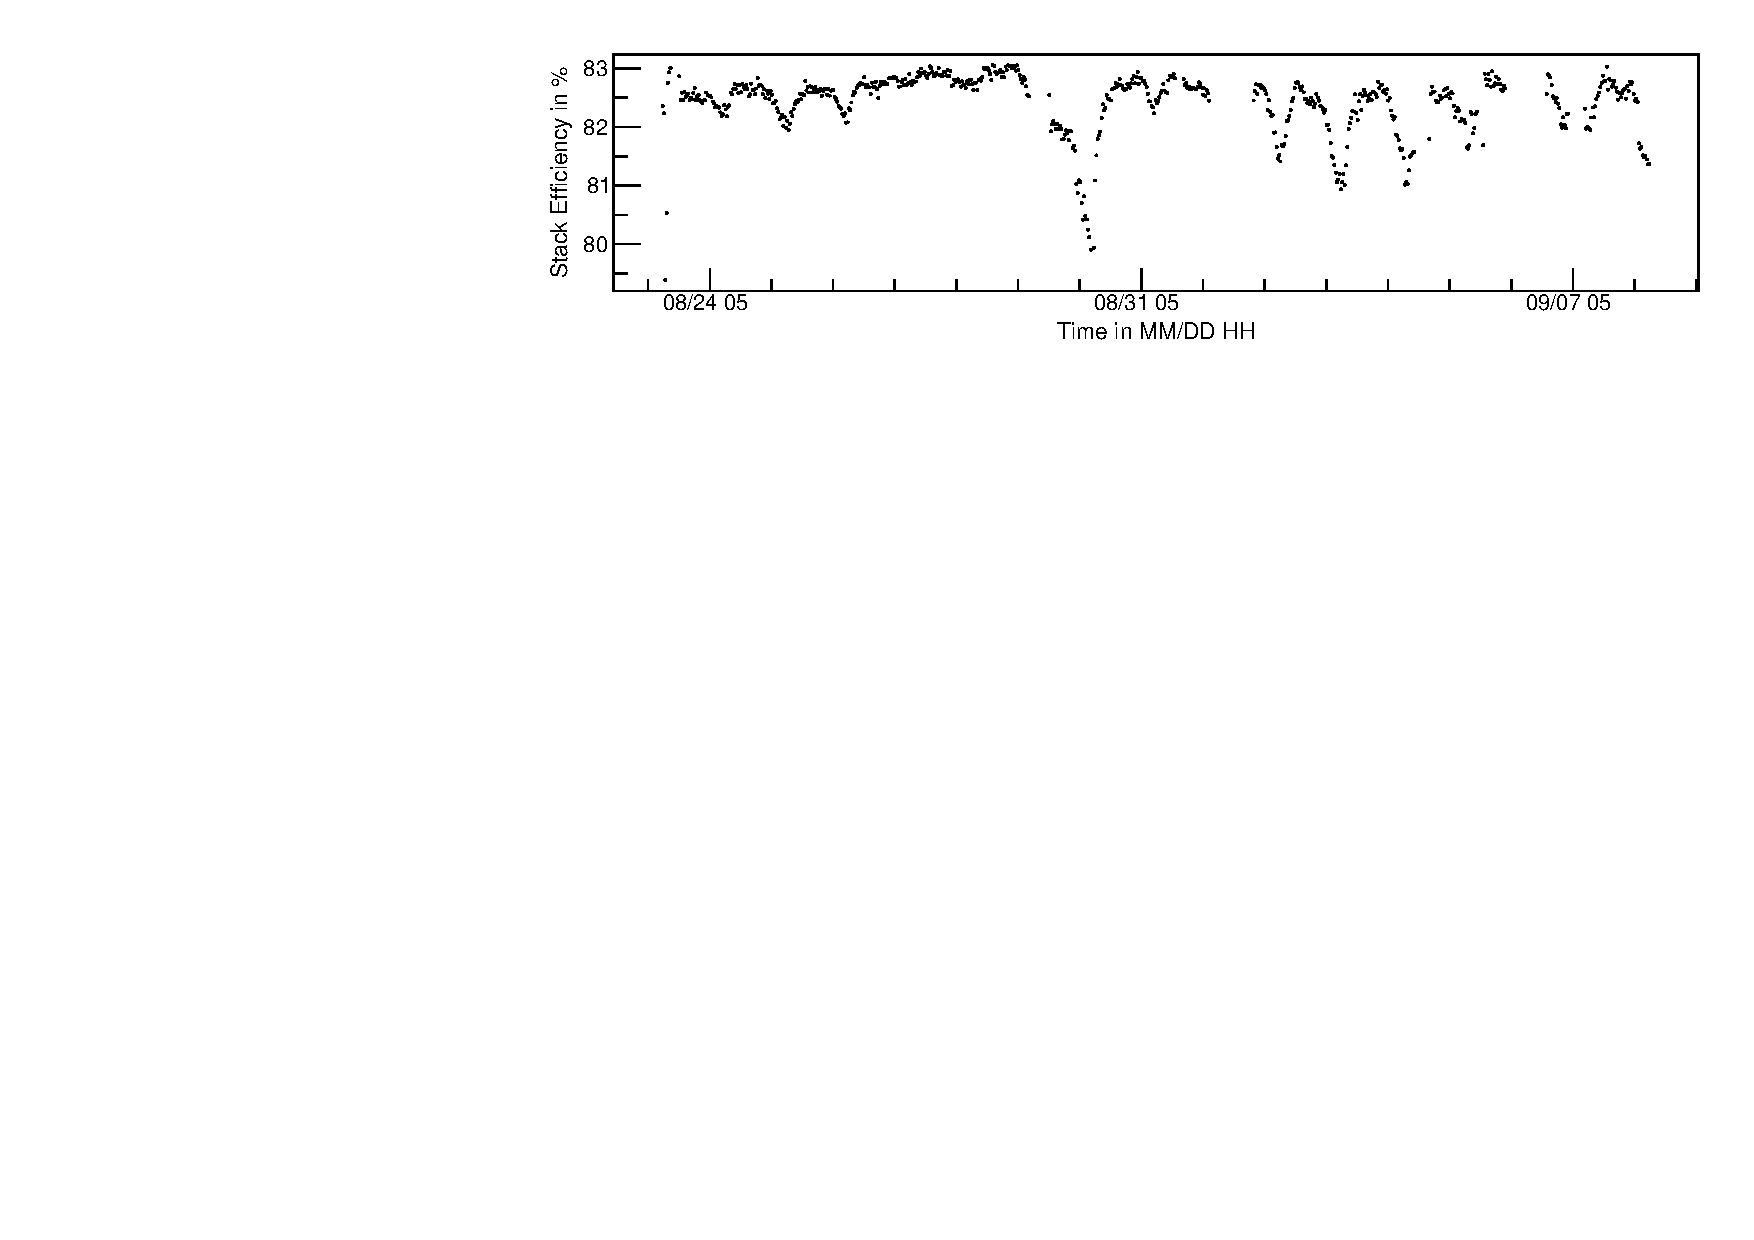
\includegraphics[width=1.0\linewidth]{stack_ineffi_1.pdf} 
  \caption{Variation of reconstruction efficiency of the detector
    with time.}
  \label{fig:stackineffi}
\end{figure}
It can be observed that the reconstruction efficiency varies
periodically with time which is correlated to the variation
of the ambient pressure and temperature due to the solar
atmospheric tides \cite{rpcleak}. But this periodic change in 
the reconstruction efficiency does not affect the relative ratio of
the multiple track events. The pure multiple track events are
$\sim$0.01\% of triggered events. Out of the total triggered events,
also 6--7\,\% of events are due to noises and hadronic showers
initiated at the roof.
An extreme shower event (which can also be due to the noise) shown
in the Figure~\ref{fig:eshower} can also imitate a multi-track event.
\begin{figure}[h]
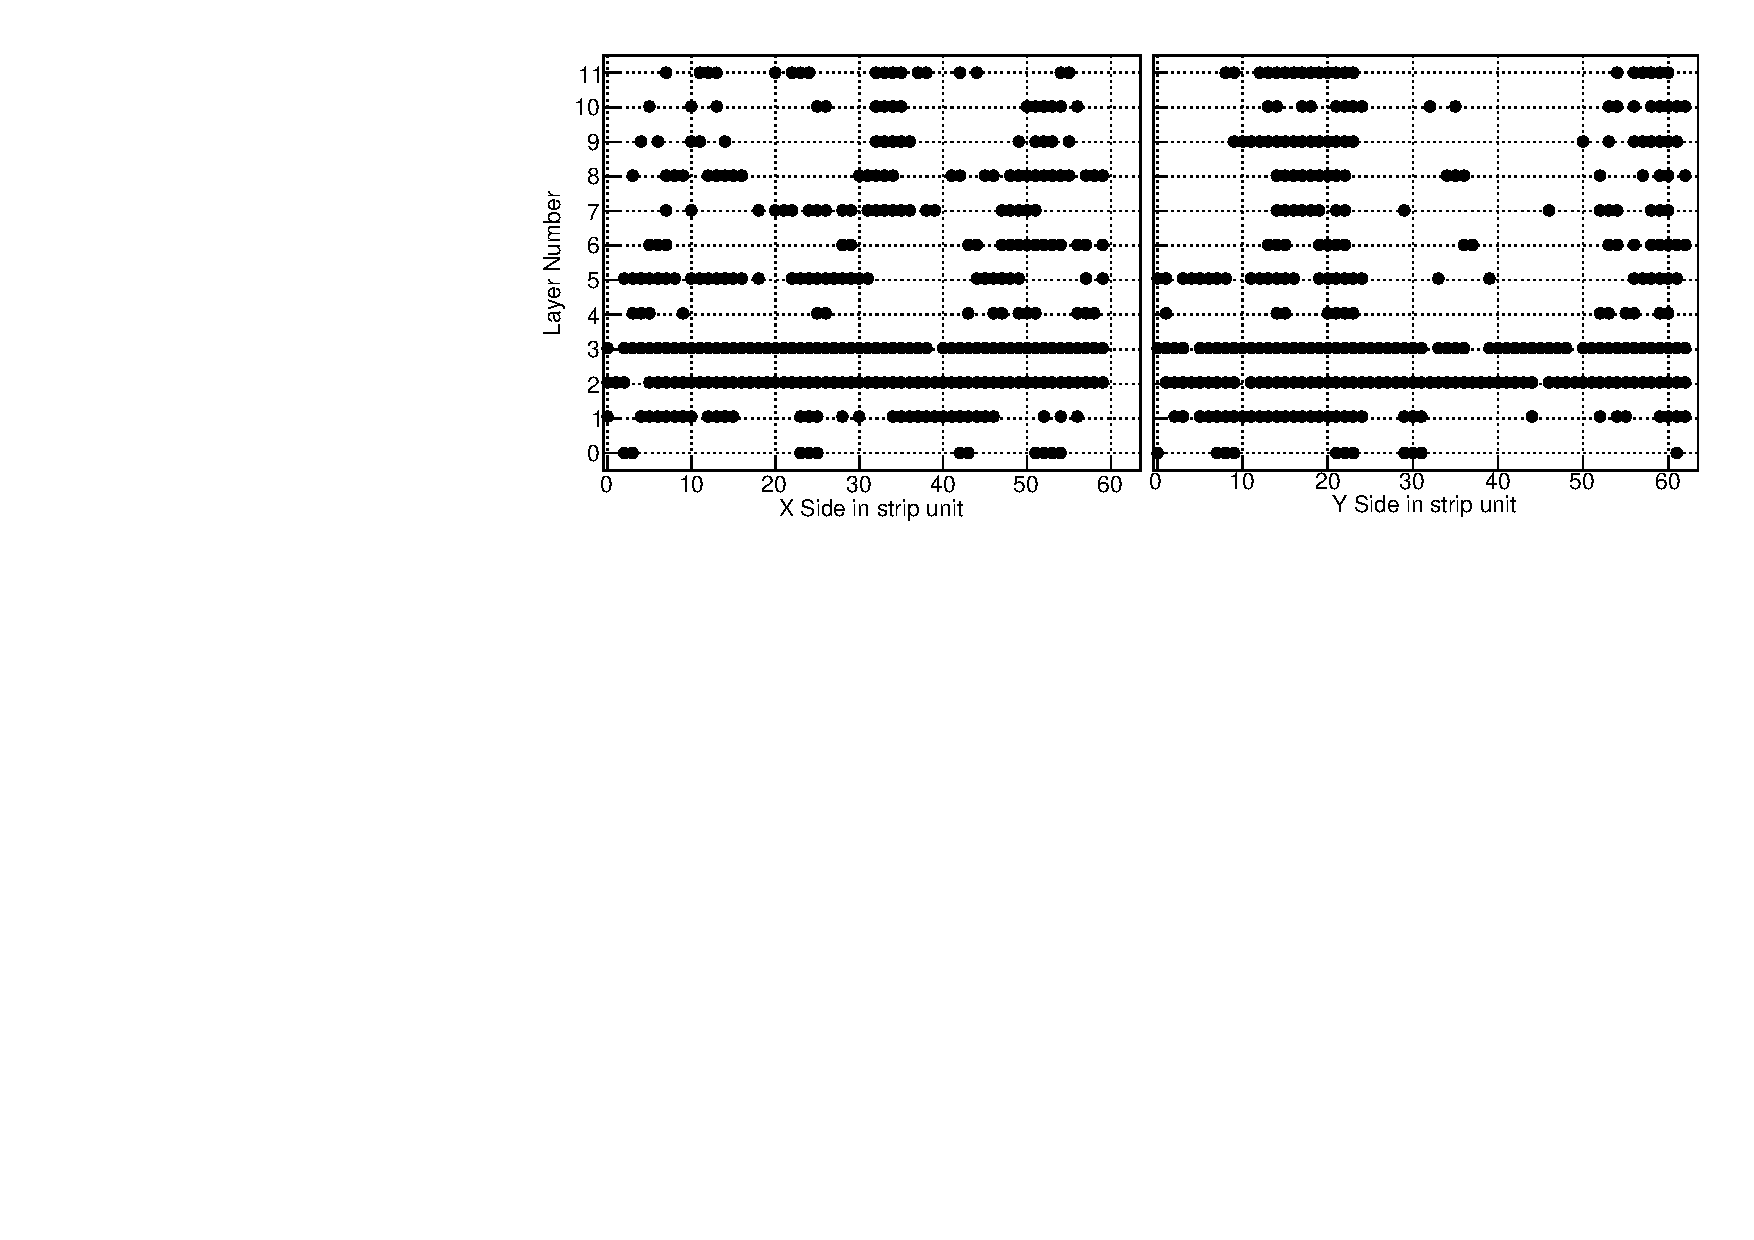
\includegraphics[width=1.0\linewidth]{Multi_Event_20170823_102605_3088_Shower_1.pdf} 
 \caption{Example of an extreme shower event.}
 \label{fig:eshower}
\end{figure}
Any such ambiguous events are rejected by the selection criteria
used in the study discussed in the following.

The zenith and azimuth angle distributions of the reconstructed
tracks are presented in the Figure \ref{fig:thetaphi}(a) and
\ref{fig:thetaphi}(b), respectively.
\begin{figure}[h]
  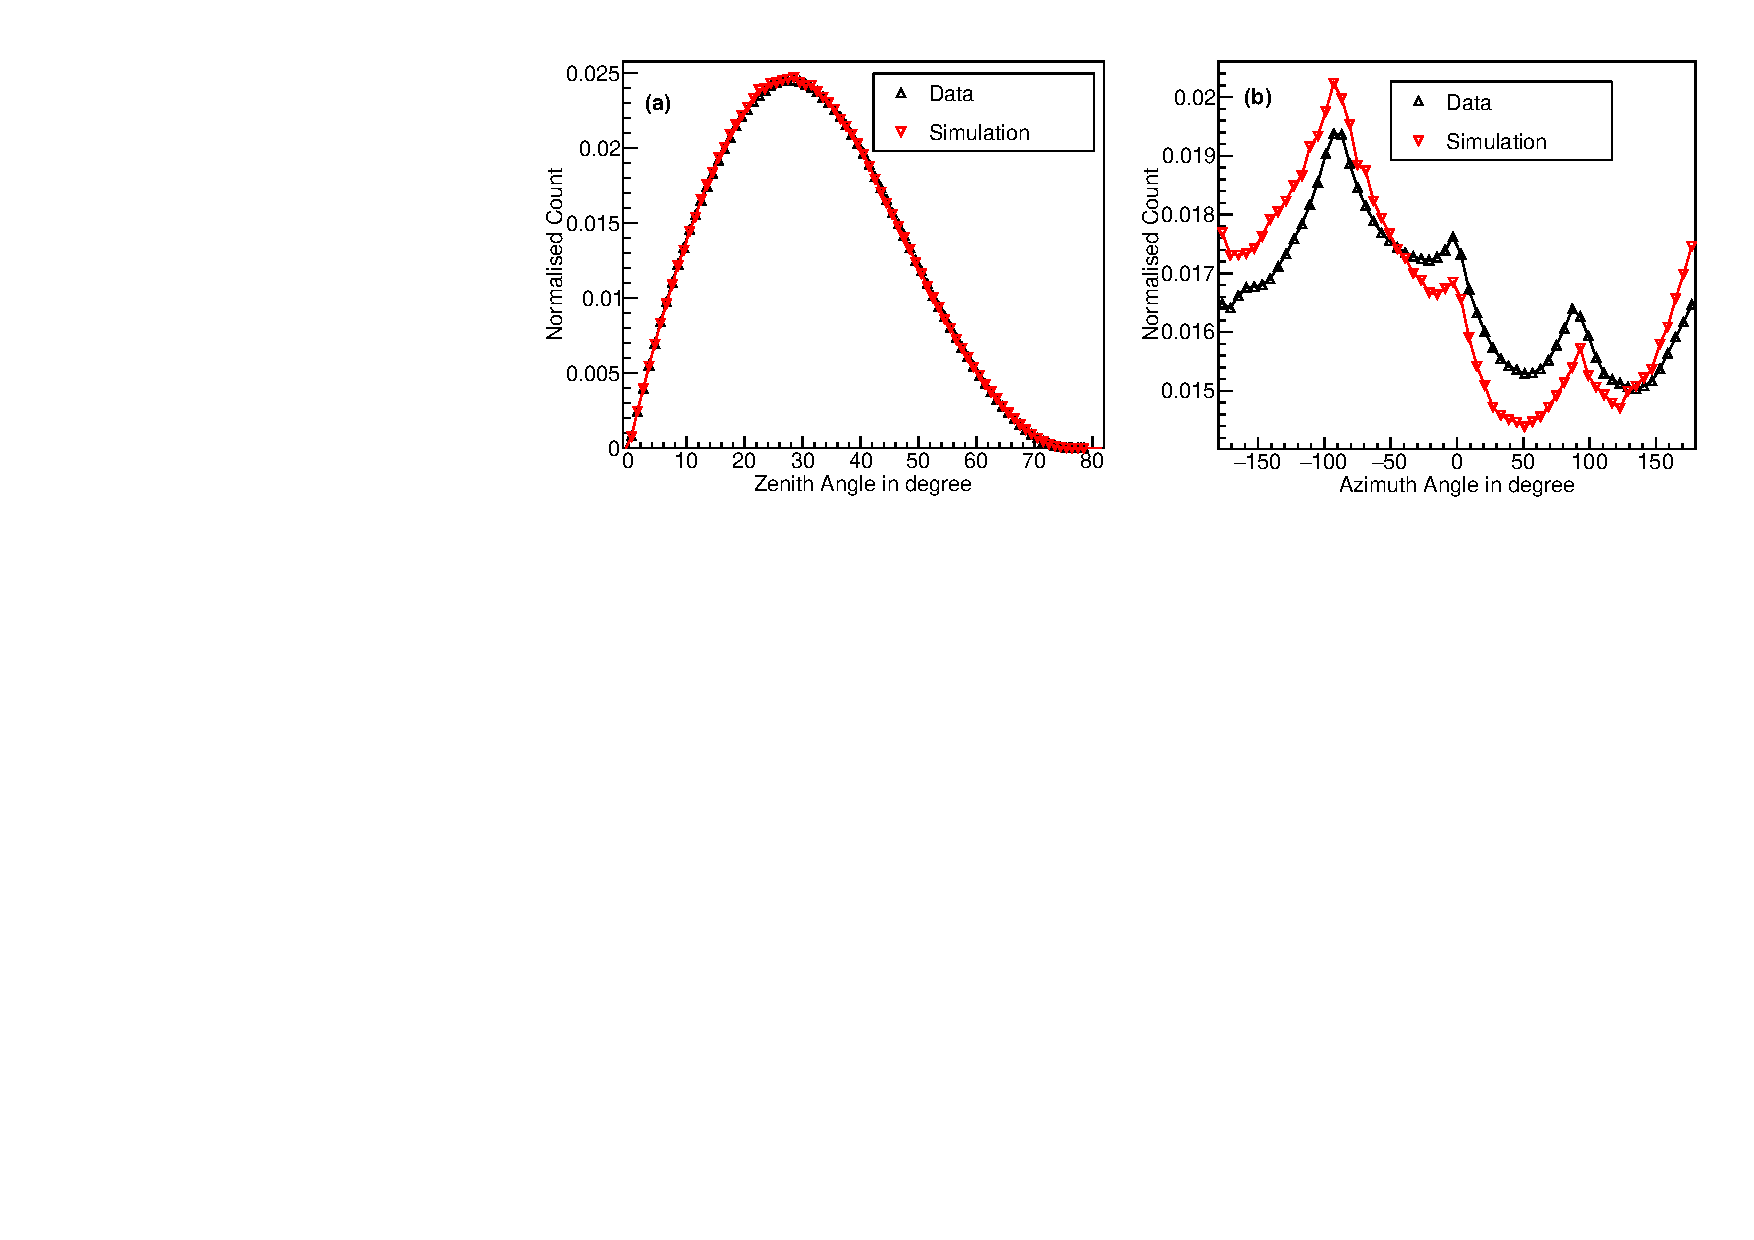
\includegraphics[width=1.0\linewidth]{thetaphi_compare_all.pdf} 
  \caption{(a) Zenith and (b) Azimuth Angle of cosmic rays
    reaching the detector 
stack.}
  \label{fig:thetaphi}
\end{figure}
The projections from both the X--Z and Y--Z planes are combined
to produce the final 3-dimensional track(s). Any ghost tracks formed
while combining are discarded by using the timing information recorded
for each strip. The events of interest for this study are the
events with more than one reconstructed 3-dimensional track.
The distribution of the time separation between each pair of
reconstructed tracks for both the simulation and data are shown in the
Figure~\ref{fig:time_sep}(a).
\begin{figure}[h]
  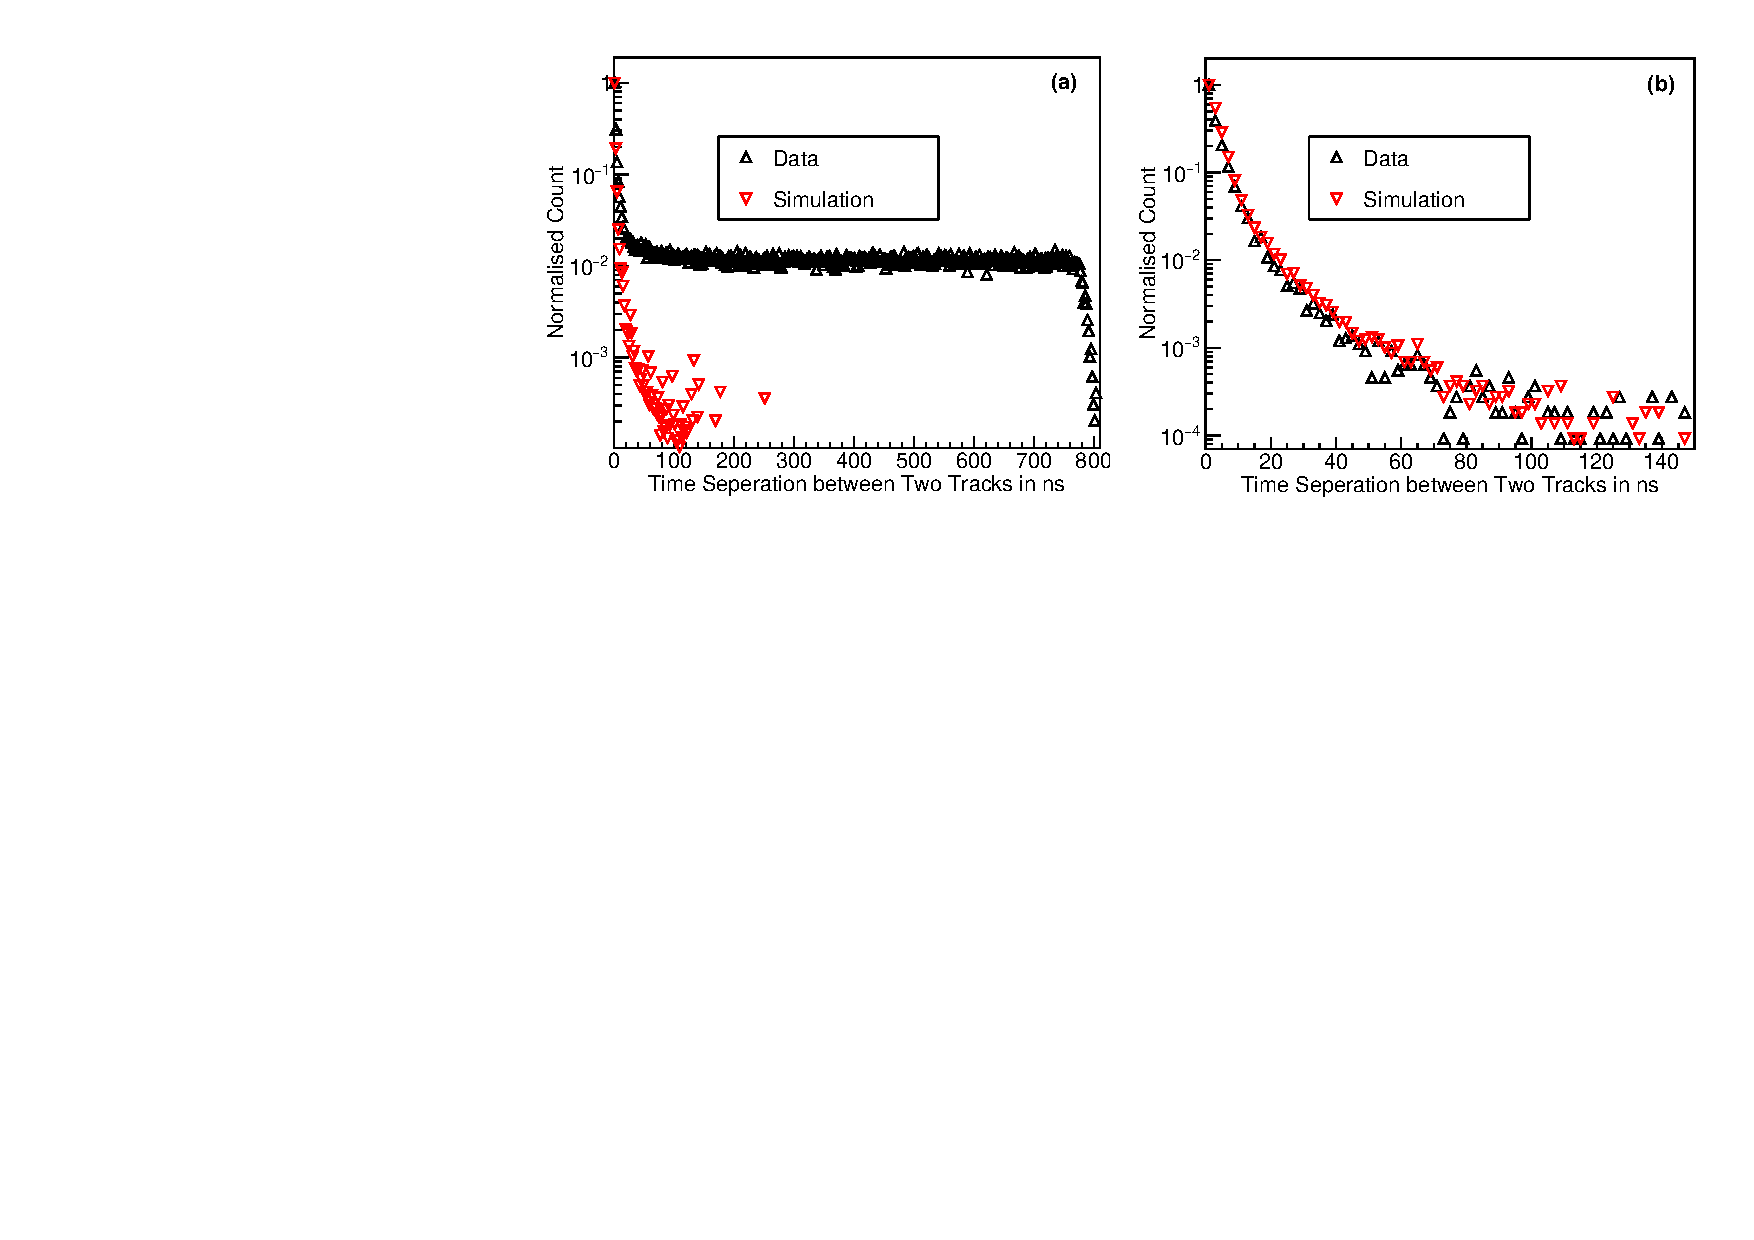
\includegraphics[width=1.0\linewidth]{time_diff_compare_all.pdf} 
  \caption{Time separation of two tracks for (a) all events and
    (b) for events with only parallel tracks.}
  \label{fig:time_sep}
\end{figure}
In the case of data, it can be observed that there is a significant
number of events where multiple particles are reaching the detector
with large relative time delay. The random coincidence of particles
originating in the different cosmic showers is the cause for these
events. The random coincidence of particles from different cosmic
showers are absent in the simulation as only one shower is simulated
at a time in the CORSIKA.
So the following procedure is adopted to reject the random
coincidences from the events which have been initiated by the same
showers.

In the simulation, it is observed that the particles originating
from the same shower are detected in the RPC stack as the parallel
tracks. This can be verified by calculating the skewed angle between
each pair of tracks reconstructed in an event. The value of
skewed angle is ideally supposed to be zero in case of the parallel
tracks, but due to the finite size of the strip width and multiple
scattering the distribution of skewed angle has finite width and tail.
%% it has finite width and tails. 
The distribution of the
skewed angle between the each pair of tracks reconstructed from
both the simulation and data is shown in the
Figure~\ref{fig:skewed_angle}(a).
\begin{figure}[h]
  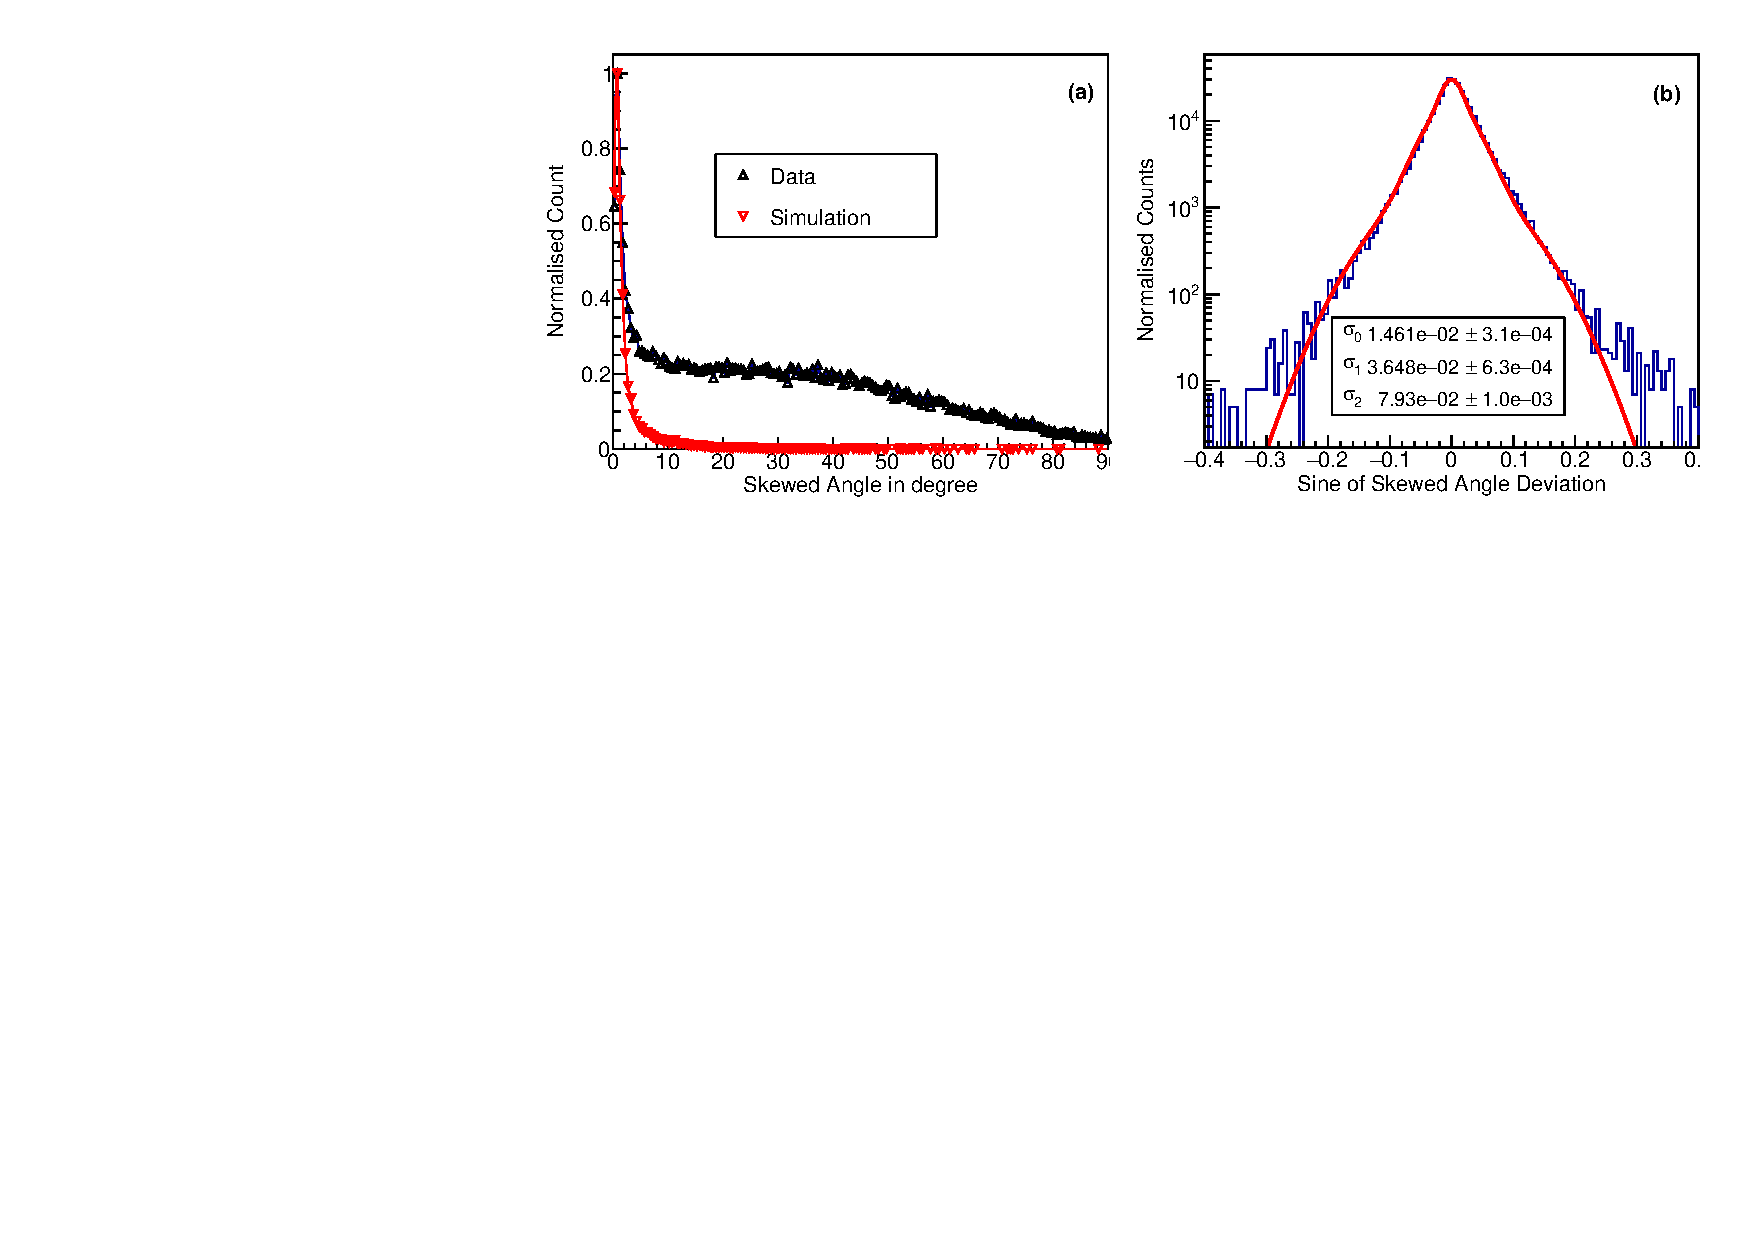
\includegraphics[width=1.0\linewidth]{skewed_compare_reso_2plot_full.pdf}
  \caption{(a) Skewed angle between two tracks originating
    outside of the detector, (b) Skewed angle difference
    between generated and reconstructed tracks fitted with
    triple-Gaussian function.}
  \label{fig:skewed_angle}
\end{figure}
Now, only the parallel tracks are of the importance in this study
because of their same origin. In order to define the parallel tracks
reconstructed in this detector setup, good understanding about the
resolution of the skewed angle is necessary. To understand the
application of the skewed angle, events with multiple particles are
simulated in the GEANT4. The skewed angle $\left(s_{gen}\right)$
between the generated pair of tracks in an event is calculated using
their generated directions. The skewed angle $\left(s_{reco}\right)$
between the same pair of tracks is estimated from the track
reconstruction also. The distribution of the sine of the difference
of the skewed angle between the generated particles and the skewed
angle between the reconstructed tracks, defined as the
$\sin\left(s_{gen}-s_{reco}\right)$, is shown in the
Figure~\ref{fig:skewed_angle}(b). This distribution is fitted with
the triple-Gaussian function. The three components of these angular
resolutions ($\sigma_{0}$, $\sigma_{1}$, $\sigma_{2}$) represent the
cases, where (0) no multiple scattering happened for the pair of
tracks, (1) one of the tracks has gone through multiple scattering and
(2) both the tracks have gone through multiple scatterings in the
detector medium or in the roof of the building where the detector is
housed, respectively.

Based on these observations, a pair of tracks with a skewed angle less
than $2.5^{\circ} \left(\approx 3\sigma_{0}\right)$ are considered as
parallel to each other. All the pairs of tracks present in a
reconstructed event have to comply with this selection criteria.
Thus, in the current study, only the parallel tracks are considered
to select the events generated due to the particles originating from
the same cosmic ray shower. The time difference between a pair of
tracks for both the simulated and observed data after the criteria of
parallel track selection is shown in the Figure~\ref{fig:time_sep}(b).
It can be observed that the events from the random coincidences
disappear after rejecting the events with non-parallel tracks.

The particles, originated in the interaction of the secondary particles
with the detector medium or the roof are also not parallel to the
interacting particles as shown in the Figure~\ref{fig:eventinside}.
This skewed angle criterion rejects these events as well.
\begin{figure}[h]
  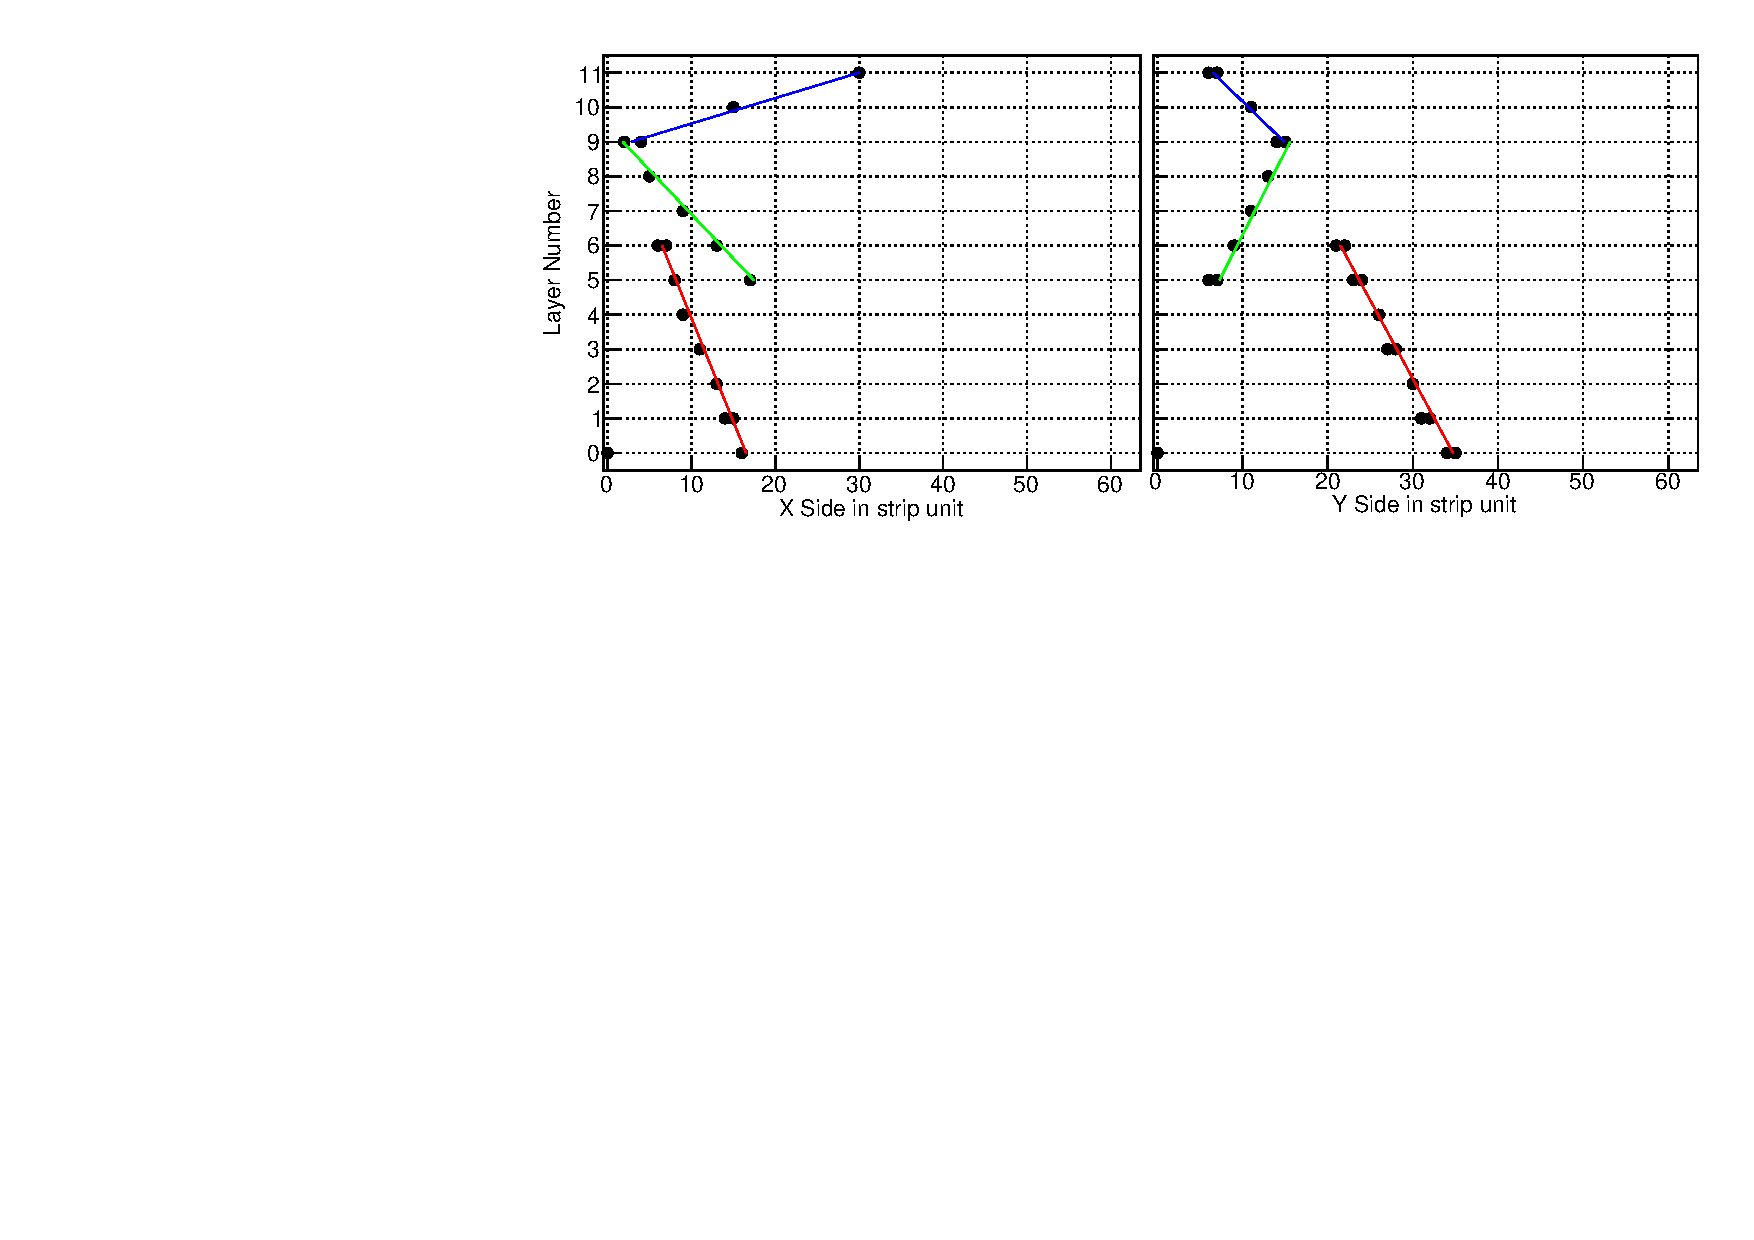
\includegraphics[width=1.0\linewidth]{Multi_Event_20170823_102605_361367_Inside_1.pdf}
  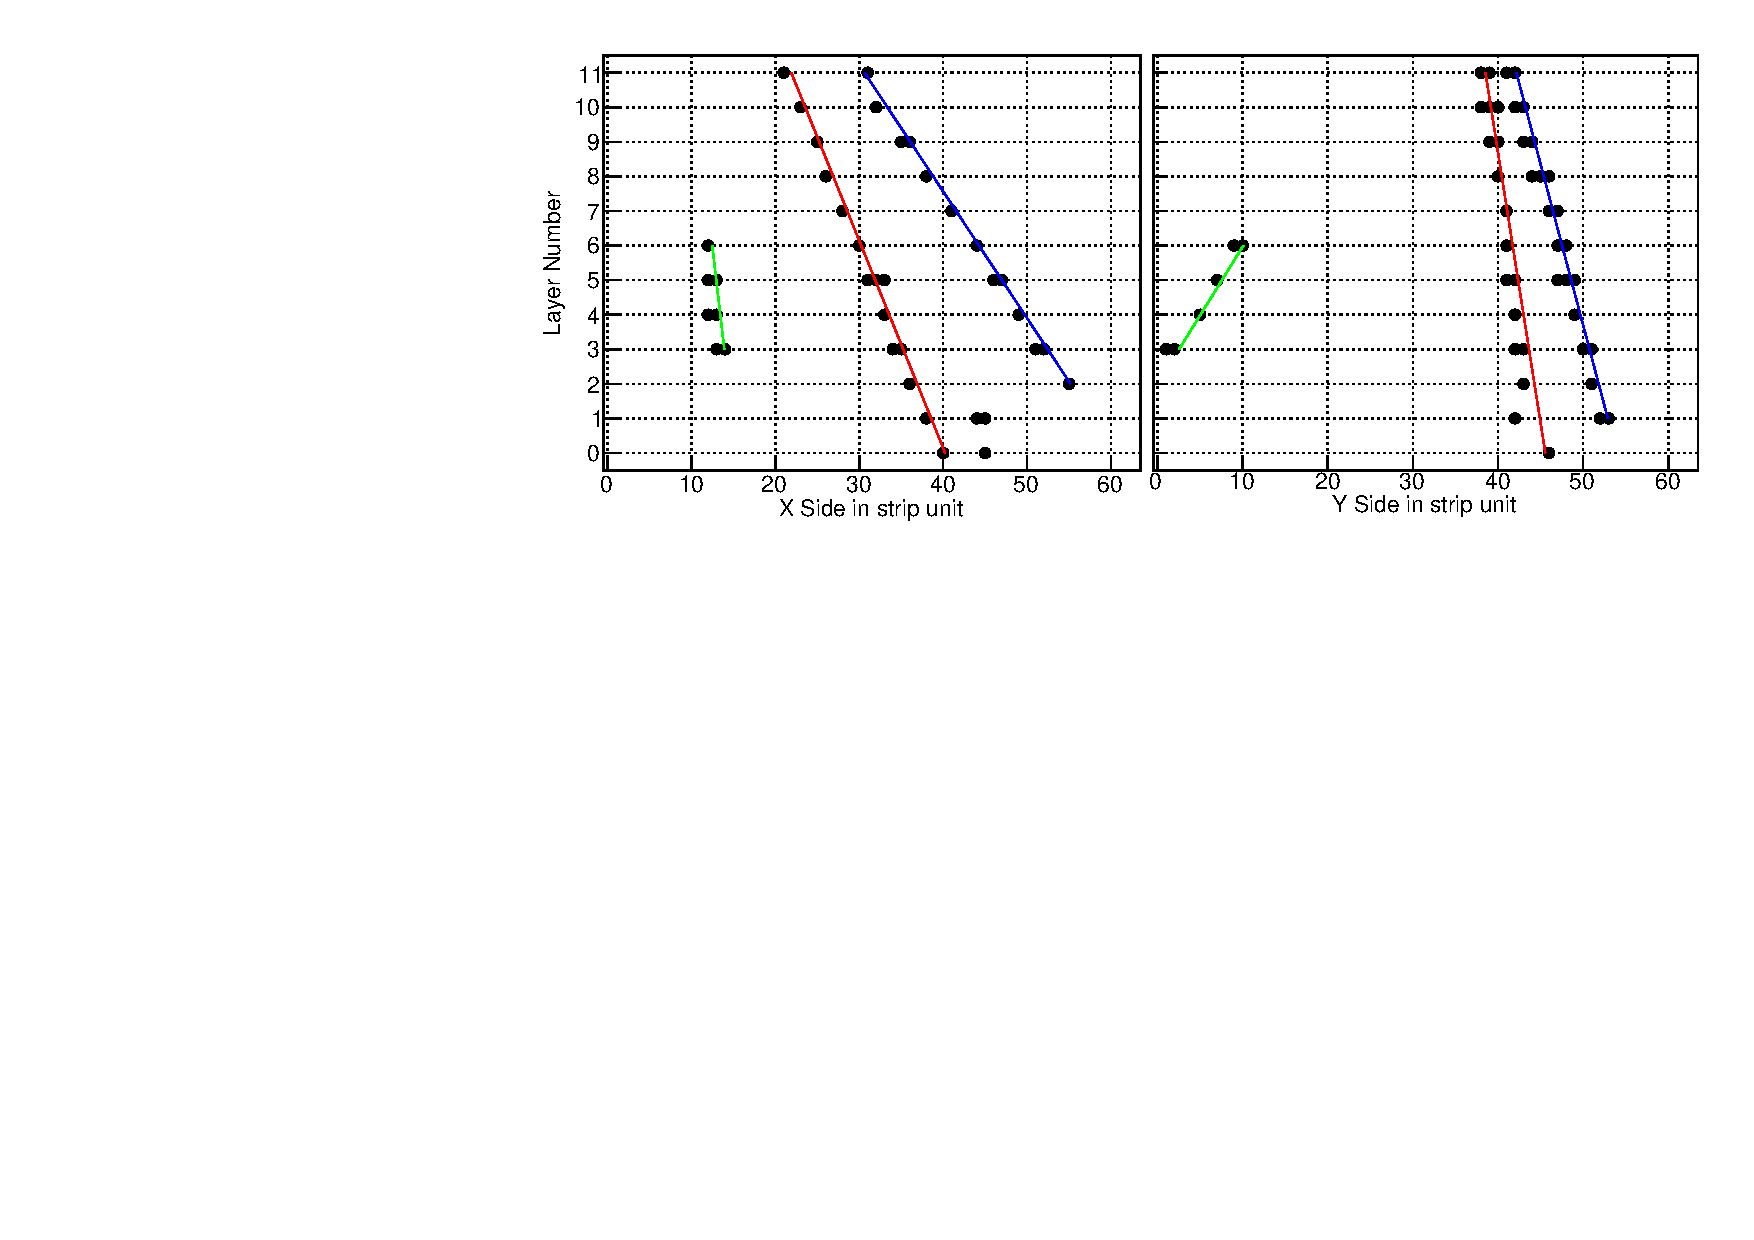
\includegraphics[width=1.0\linewidth]{Multi_Event_20170823_102605_9676_Roof_1.pdf}
  \caption{Events where the secondary cosmic ray interacted with
    the detector medium and roof generating multiple particles.}
  \label{fig:eventinside}
\end{figure}


\section{Results and Discussions} \label{sec:result}
In the present work, the event direction is presumed as a mean
direction of all individual tracks in an event. In the study, the
clustering of events towards any specific region in the sky was
not observed for the data recorded in the detector,
which can be confirmed by the Figure~\ref{fig:pinsk}.
\begin{figure}[h]
  \centering
  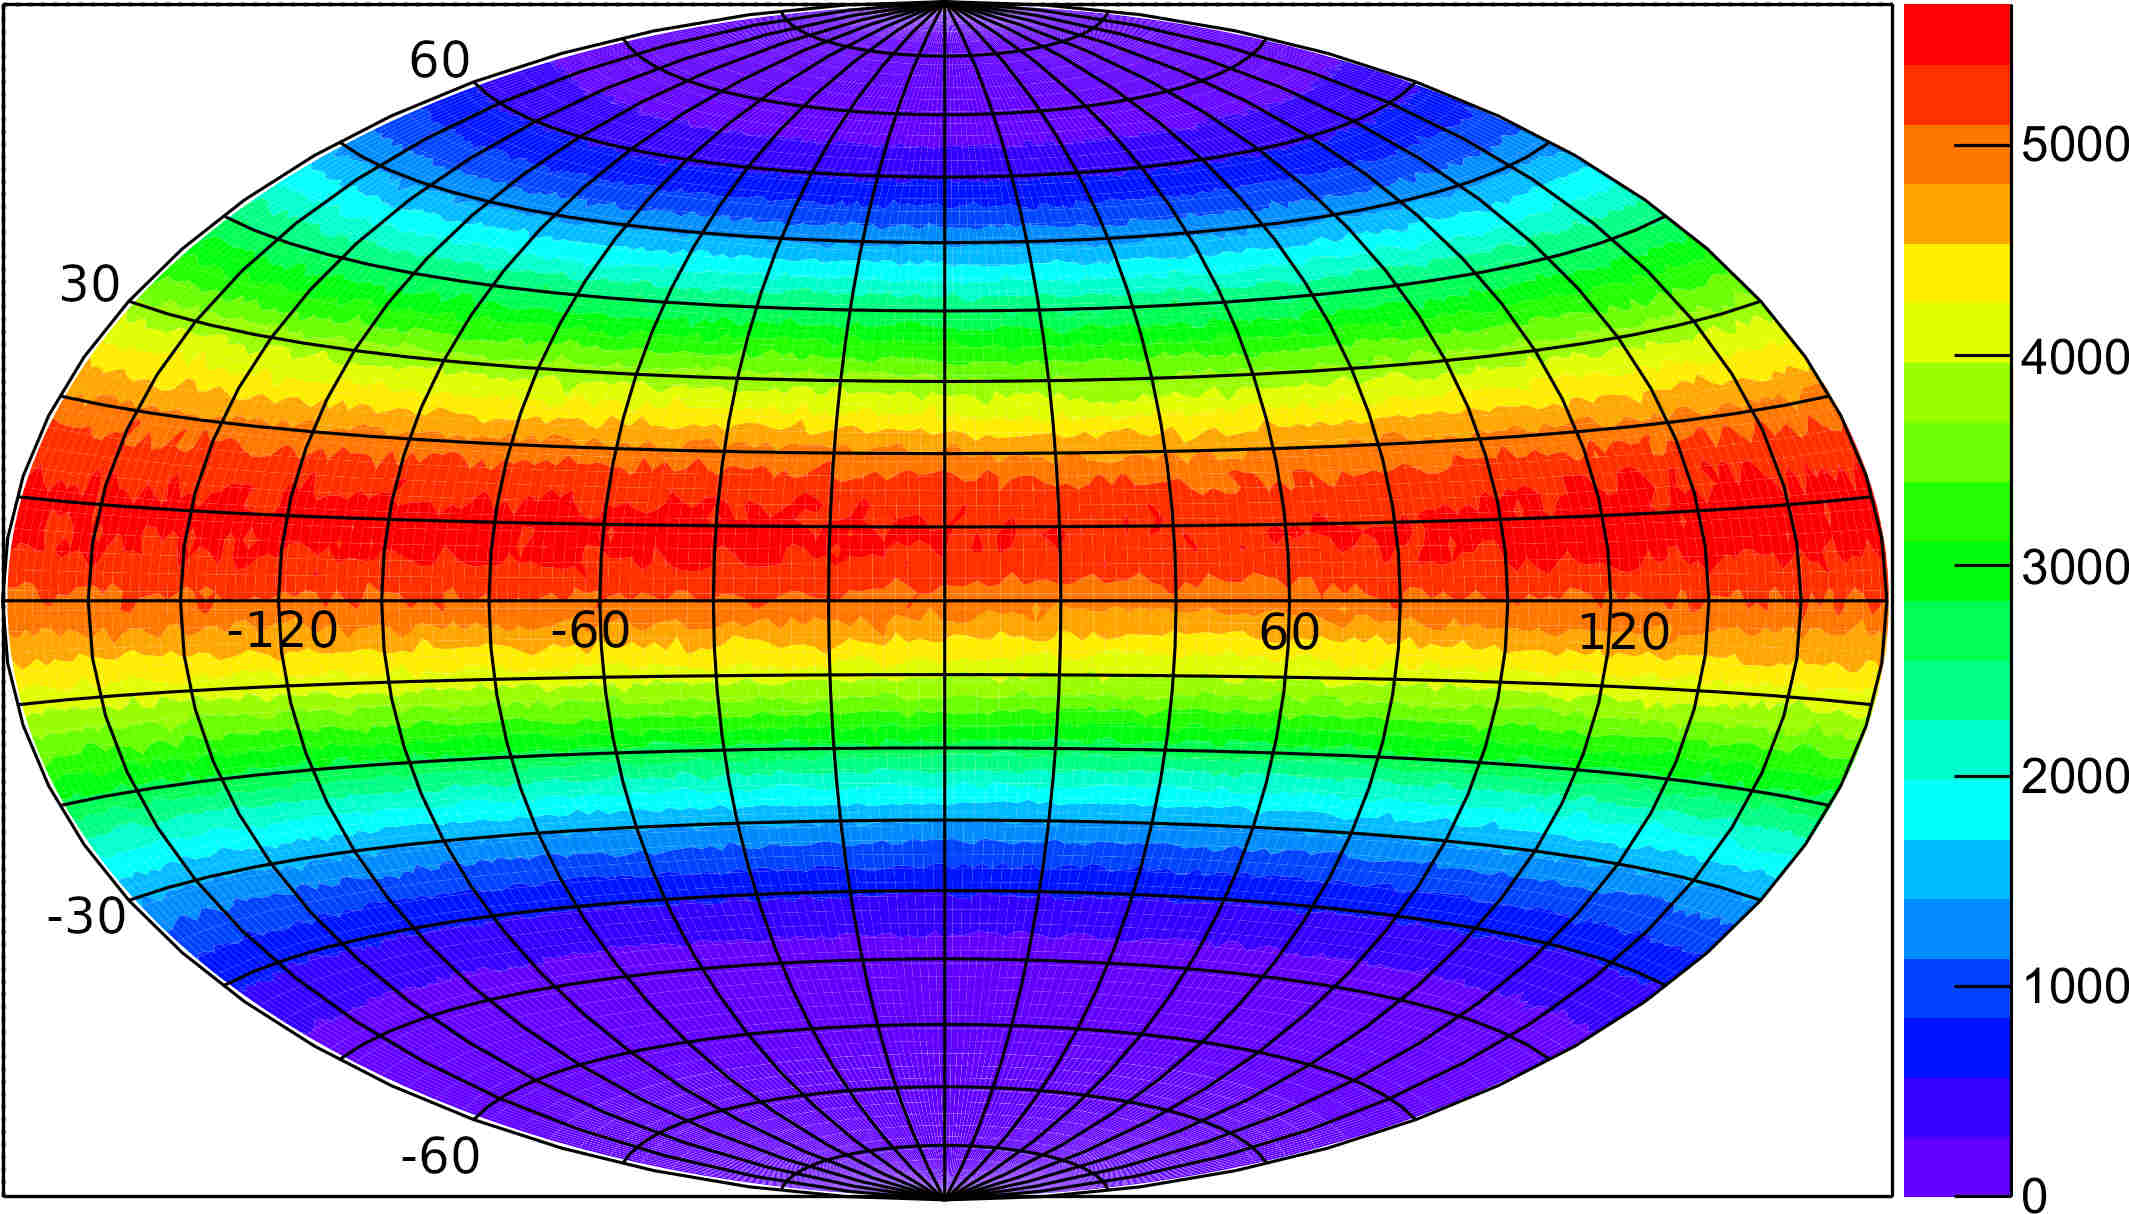
\includegraphics[width=0.85\linewidth]{point_in_sky.jpg} 
  \caption{Reconstructed direction of the tracks in the detector observed for the
    data recorded in the detector.}
  \label{fig:pinsk}
\end{figure}
Also, no significant
modulation of the fractions of multiple track events was observed
during the period of observation irrespective of periodic changes
in trigger rate. 
Hence, the assumption of the uniform distribution of the cosmic ray
directions which are used in the CORSIKA simulations are justified
by the absence of anisotropy in the data.

The total number of events with at least one reconstructed track in it
is approximately 206\,millions.
The normalised fraction of the events containing 2, 3 and 4 tracks
with respect to single track events are calculated to be
$6.35\pm 0.05\times 10^{-5}$, $5.82\pm 0.53\times 10^{-7}$ and
$1.94\pm 0.97\times 10^{-8}$, respectively from the cosmic ray data.

The normalised fraction of the events containing 2, 3 and 4 tracks
are also calculated from the CORSIKA simulation for different types
of cosmic primaries (H, He, C, O, Si, and Fe) and for different
hadronic interaction models (QGSJET-II-04 and QGSJET01d), which are
shown in the Table~\ref{tab:ratio1}. In order to compare the simulated
results with data, all the normalised fraction, calculated for
different cosmic primaries are summed with weights where the
abundances in the primary composition\cite{cosmic1,pdgspectra1} are
used as the weights. The
comparison of the data and the combined predictions are given in
the Table~\ref{tab:ratio2}.

\begin{table}[btbp]
% \centering
 \scalebox{0.7}{
  \begin{tabular}{|c|cccccc|} \hline
   No of   &  H      & He       & C     & O    & Si      & Fe   \\  \cline{2-7}
   Tracks  & \multicolumn{6}{c|}{QGSJET-II-04}                 \\ \hline
          2      & $2.19\pm 0.12\times 10^{-5}$  & $4.71\pm 0.19\times 10^{-5}$ & $1.21\pm 0.02\times 10^{-4}$ & $1.61\pm 0.02\times 10^{-4}$ & $2.42\pm 0.02\times 10^{-4}$ & $4.58\pm 0.03\times 10^{-4}$ \\
          3      & $1.02\pm 0.12\times 10^{-7}$ & $3.04\pm 0.17\times 10^{-7}$ & $1.78\pm 0.05\times 10^{-6}$  & $3.11\pm 0.06\times 10^{-6}$ & $5.57\pm 0.08\times 10^{-6}$ & $1.61\pm 0.02\times 10^{-5}$ \\
          4      & $1.61\pm 0.65\times 10^{-9}$ & $8.80\pm 2.46\times 10^{-9}$ & $5.83\pm 0.47\times 10^{-8}$  & $1.12\pm 0.07\times 10^{-7}$ & $2.35\pm 0.11\times 10^{-7}$ & $1.02\pm 0.03\times 10^{-6}$ \\
\hline
                 & \multicolumn{6}{c|}{QGSJET01d}                     \\ \hline
          2      & $2.14\pm 0.12\times 10^{-5}$ & $4.74\pm 0.13\times 10^{-5}$ & $1.19\pm 0.02\times 10^{-4}$  & $1.52\pm 0.02\times 10^{-4}$ & $2.50\pm 0.02\times 10^{-4}$ & $4.56\pm 0.03\times 10^{-4}$ \\
          3      & $9.13\pm 1.22\times 10^{-8}$ & $3.91\pm 0.18\times 10^{-7}$ & $1.90\pm 0.04\times 10^{-6}$  & $3.14\pm 0.08\times 10^{-6}$ & $6.19\pm 0.07\times 10^{-6}$ & $1.65\pm 0.02\times 10^{-5}$ \\
          4      & $0.75\pm 0.38\times 10^{-9}$& $6.48\pm 1.38\times 10^{-9}$ & $6.00\pm 0.43\times 10^{-8}$  & $1.07\pm 0.07\times 10^{-7}$ & $3.39\pm 0.11\times 10^{-7}$ & $1.16\pm 0.03\times 10^{-6}$ \\ \hline
\end{tabular}}
 \caption{Fraction of track with 2, 3 and 4 tracks obtained from
   Simulation for different primaries (H, He, C, O, Si and Fe) and
   different physics packages 
   (QGSJET-II-04 and QGSJET01d).}\label{tab:ratio1}
\end{table}

\begin{table}[btbp]
  \centering
\begin{tabular}{|c|ccc|} \hline
No of Tracks &  Data &   QGSJET-II-04     &  QGSJET01d \\ \hline
    2         & $6.35\pm 0.05\times 10^{-5}$ & $2.35\pm 0.13\times 10^{-5}$ & $2.37\pm 0.12\times 10^{-5}$ \\
    3         & $5.82\pm 0.53\times 10^{-7}$ & $1.12\pm 0.13\times 10^{-7}$ & $1.23\pm 0.13\times 10^{-7}$ \\
    4         & $1.94\pm 0.97\times 10^{-8}$ & $3.21\pm 0.87\times 10^{-9}$ & $2.43\pm 0.50\times 10^{-9}$ \\ \hline
\end{tabular}
\caption{Comparison of track fraction with 2, 3 and 4 tracks
  obtained from Data and simulation, with combined fractions
  as par abundances of cosmic ray particles.}\label{tab:ratio2}
\end{table}

If the abundances of elements in the primary cosmic ray spectrum as
observed in \cite{cosmic1,pdgspectra1} are used to estimate the final
results from simulation, the normalised track fractions of the events
containing 2, 3 and 4 tracks are order of magnitude less than
the data. The systematic error due to the uncertainties of roof
thickness, material in the detector setup, strip multiplicity, noise
and efficiencies are much smaller than the observed discrepancy
between data and MC prediction. These results clearly demonstrate
that there is a discrepancy between the observed data and 
predictions from cosmic ray particle spectrum, the CORSIKA and
finally the GEANT4 simulation.

A few other experiments (KGF\cite{kgf1}, ALICE\cite{alice1},
MACRO\cite{macro1}, DELPHI\cite{delphi1}, ALEPH\cite{aleph1},
KASCADE-Grande\cite{kascade1}, etc.) have also studied the multi-muon
tracks in the cosmic events in the respective detectors. Except for
the KASCADE-Grande, all other experiments were performed under
the ground. The underground experiments have observed events with
large multiplicities because of the large size of the detectors and
the overburden of rock and soil, which block showers with low energy.
The multiplicity of the cosmic ray particles observed in a detector
is highly dependent on the dimensions, aperture, energy threshold
and the detector's location. Hence, it is difficult to compare the
results of the aforesaid experiments quantitatively with the
small-scale detectors setup in this current study. But all
the studies based on the aforesaid experiments have also indicated
a similar discrepancy between the CORSIKA spectra and the observed
data. The KASCADE-Grande experiment has also concluded that the
attenuation length of muons in the atmosphere from the simulation
is much smaller than estimation from the observed data\cite{kascade1}.

Although, the bulk of primary particles interacts at center-of-mass
energies far below 10\,GeV \cite{corsika763}, it is observed in the
simulation that a significant amount of primaries which are
responsible for higher particle multiplicities in the present setup,
are in the range beyond the scope of the present collider experiments.
The major problem of the EAS simulation programs is the extrapolation
of the hadronic interactions in the high energy range which is not
covered by the experimental data. The limitation of the experiments
in measuring the hadronic interactions at this high energy is mainly
due to the limitation of the design of high energy $p\bar{p}$-colliders
\cite{corsika763}. In the present $p\bar{p}$- or $p\,p$-colliders, the
forward direction is not accessible. The secondary particles which are
of the higher importance in the development of EAS programs are
undetected in the beam pipe of the colliders. The largest energy
fraction of each $p\bar{p}$-collision is carried away by these
particles.
The maximum attainable energy in these colliders is much lower than
those found in cosmic rays. Therefore, the extrapolations based on
theoretical models are mainly used by all the EAS programs.
While, the energy of the cosmic rays contributing for the single track
events in the current detector setups are well within the boundary of
the current physics models (up-to $\sim$1\,TeV), a significant amount
of the interactions contributing for the higher multiplicities are
beyond this energy and are not supported by the experimental
data \cite{corsika763}.

\section{Chapter Summary}
An experimental setup consisting of 12 layers of glass RPCs of the size
of 2\,m\,$\times$\,2\,m has been built at IICHEP-Madurai. The cosmic
ray data recorded by this detector setup is used to analyse the
secondary cosmic rays reaching the surface of the earth. In this
current study, we probed the multiplicity of the particles passing
through the detector. The recorded data is compared with the
Monte-Carlo simulations.
In the period between August 23, 2017 to September 8, 2017,
approximately two hundred million cosmic ray events were recorded.
As it is shown above, the analysis showed a discrepancy in the
result predicted by the EAS simulation program which can be observed
in the comparison of the track multiplicity between the data and
Monte-Carlo. The results of the current study reflect that the current
physics models of interactions at the earth's atmosphere are unable to
reproduce the air showers accurately. The earlier measurements of the
muon multiplicity along with the present result can be used to
improve the parameters of the hadronic models at the high energies
and/or the cosmic ray spectral index along with the composition of the
primary cosmic rays.
